\chapter{Analisis}
\label{chap:analisis}

Pada bab ini akan dijelaskan mengenai analisis Portal Akademik Mahasiswa, analisis SIAKAD, analisis data yang dibutuhkan untuk \textit{screensaver}, serta analisis sistem \textit{screensaver}.

\section{Analisis Portal Akademik Mahasiswa}
\label{analisisPemanfaatanJsoup}
Untuk mengambil data mahasiswa, diperlukan sumber data mahasiswa tersebut. Sumber data mahasiswa tersebut dapat diperoleh melalui Portal Akademik Mahasiswa. Portal Akademik Mahasiswa merupakan sebuah situs yang diperuntukkan bagi mahasiswa untuk mendapatkan informasi mengenai profil dan kegiatan akademik mahasiswa tersebut. Mahasiswa dapat mengakses Portal Akademik Mahasiswa melalui \textit{URL} \url{https://studentportal.unpar.ac.id/}. Untuk mengakses Portal Akademik Mahasiswa, mahasiswa harus melakukan \textit{login} menggunakan \textit{email} dan \textit{password} mahasiswa tersebut.

Aplikasi \textit{screensaver} akan melakukan \textit{http request} ke Portal Akademik Mahasiswa untuk mendapatkan data untuk setiap kebutuhan dari masing-masing fitur yang ada, dimana fitur-fitur yang terdapat dalam aplikasi Mahasiswa Wali \textit{Screensaver} adalah informasi umum mengenai mahasiswa, serta prestasi akademik mahasiswa. Pengambilan data secara langsung dari Portal Akademik Mahasiswa dilakukan menggunakan \textit{library} jsoup. Beberapa implementasi pemanfaatan jsoup untuk mengambil data-data tersebut sudah diimplementasikan pada skripsi Andrianto Sugiarto \cite{ifstupor} sebelumnya. Data yang telah didapat dari Portal Akademik Mahasiswa kemudian diolah ke dalam SIAModels, dan ditampilkan sesuai dengan fitur-fitur yang ada pada aplikasi Mahasiswa Wali \textit{Screensaver}.

% @@ -66,7 +66,6 @@ public class Scraper {
%      public void init() throws IOException {
%          Connection baseConn = Jsoup.connect(BASE_URL);
%          baseConn.timeout(0);
% -        baseConn.validateTLSCertificates(false);
%          baseConn.method(Connection.Method.GET);
%          baseConn.execute();
%      }

\subsection{\textit{Login}}
Halaman \textit{Login} (Gambar \ref{fig:3_login} dan \ref{fig:3_login_2}) merupakan halaman dimana mahasiswa memasukkan \textit{email} dan \textit{password} untuk mengakses menu-menu Portal Akademik Mahasiswa.

\begin{figure}[H]
	\centering
	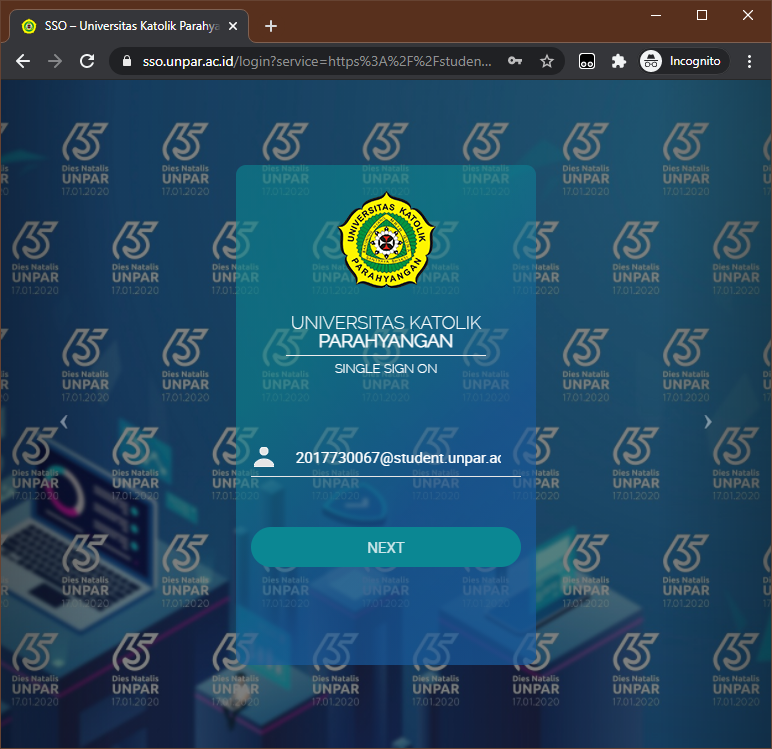
\includegraphics[scale=0.45]{Gambar/login_2.png}
	\caption{Halaman \textit{Login} 1} 
	\label{fig:3_login}
\end{figure}

\begin{figure}[H]
	\centering
	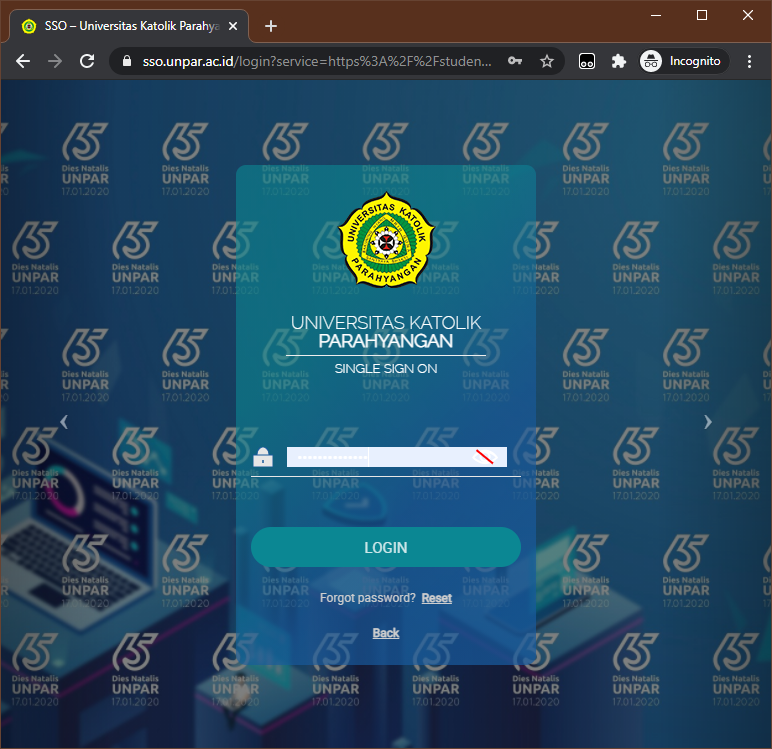
\includegraphics[scale=0.45]{Gambar/login_3.png}
	\caption{Halaman \textit{Login} 2} 
	\label{fig:3_login_2}
\end{figure}

\textit{Login} dilakukan dengan mengirim \textit{request method} POST, dan kemudian mengambil session yang akan digunakan sebagai \textit{cookies} apabila \textit{login} berhasil.
Terdapat beberapa perubahan yang terjadi pada situs Portal Akademik Mahasiswa semenjak skripsi Andrianto Sugiarto \cite{ifstupor}, yang mengakibatkan perlunya perubahan (Kode \ref{diff_login}) terhadap implementasi jsoup:

\begin{enumerate}
    \item Menghapus pemanggilan fungsi validateTLSCertificates() dikarenakan sudah \textit{deprecated} \cite{jsoup}.
    \item Menghapus pengambilan data dengan kueri css \texttt{"input[name=lt]"} dikarenakan kueri tersebut sudah dihapus oleh Portal Akademik Mahasiswa.
    \item Menghapus \textit{form data} dengan \textit{key} \texttt{"submit"} yang memiliki \textit{value} \texttt{""}.
\end{enumerate}

\begin{lstlisting}[language=diff, caption=Perubahan Implementasi Jsoup Login, label=diff_login]
@@ -78,11 +77,9 @@ public class Scraper {
         Connection conn = Jsoup.connect(LOGIN_URL);
         conn.data("Submit", "Login");
         conn.timeout(0);
-        conn.validateTLSCertificates(false);
         conn.method(Connection.Method.POST);
         Response resp = conn.execute();
         Document doc = resp.parse();
-        String lt = doc.select("input[name=lt]").val();
         String execution = doc.select("input[name=execution]").val();
         String jsessionid = resp.cookie("JSESSIONID");
         /* SSO LOGIN */
@@ -90,12 +87,9 @@ public class Scraper {
         loginConn.cookies(resp.cookies());
         loginConn.data("username", user);
         loginConn.data("password", pass);
-        loginConn.data("lt", lt);
         loginConn.data("execution", execution);
         loginConn.data("_eventId", "submit");
-        loginConn.data("submit", "");
         loginConn.timeout(0);
-        loginConn.validateTLSCertificates(false);
         loginConn.method(Connection.Method.POST);
         resp = loginConn.execute();
         if (resp.body().contains(user)) {
\end{lstlisting}

\subsection{Halaman Utama}
Pada Halaman Utama Portal Akademik Mahasiswa (Gambar \ref{fig:3_home}) terdapat beberapa menu yang dapat digunakan sebagai sumber data.

\begin{figure}[H]
	\centering
	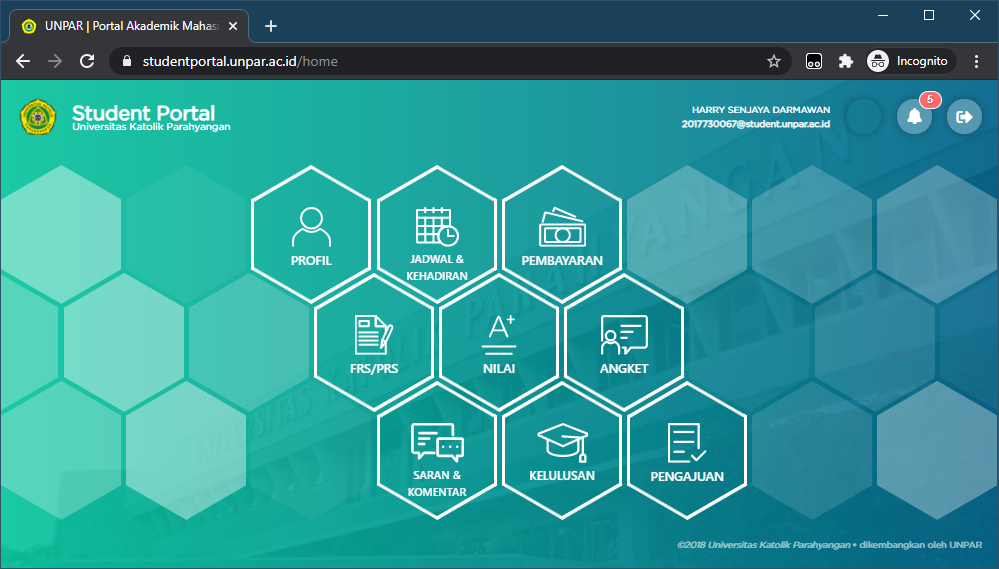
\includegraphics[scale=0.5]{Gambar/home.png}
	\caption{Halaman Utama Portal Akademik Mahasiswa} 
	\label{fig:3_home}
\end{figure}


\subsection{Profil}
    Menu Profil merupakan halaman yang menampilkan data diri mahasiswa (Gambar \ref{fig:3_profil}). 
    \begin{figure}[H]
    	\centering
    	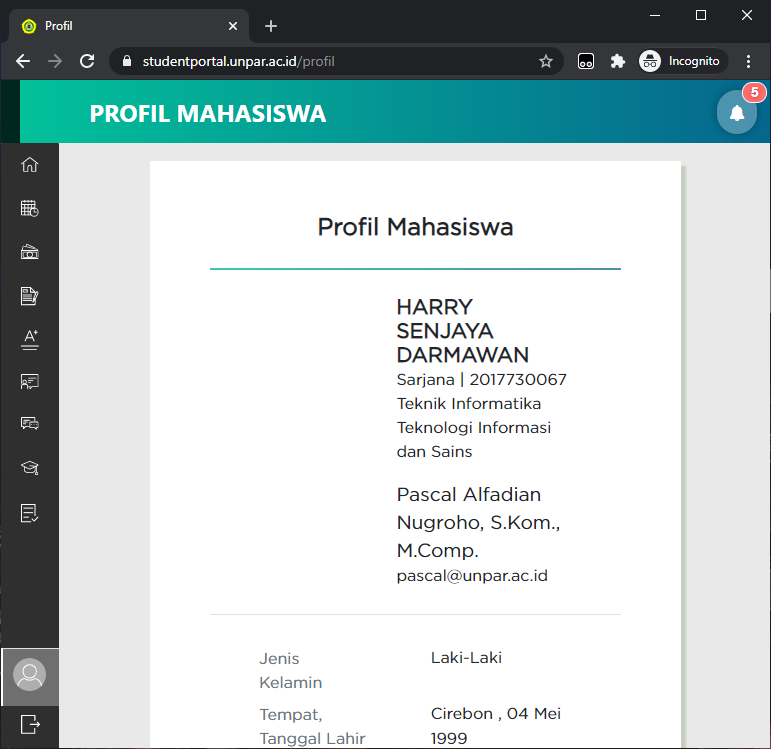
\includegraphics[scale=0.45]{Gambar/profil.png}
    	\caption{Halaman Profil} 
    	\label{fig:3_profil}
    \end{figure}

\subsection{Jadwal}
    Menu Jadwal terdiri dari beberapa submenu:
		\begin{itemize}
		    \item Kehadiran\\
		    Submenu ini berfungsi untuk menandakan kehadiran mahasiswa di suatu mata kuliah pada hari dimana mahasiswa tersebut mengakses halaman tersebut (Gambar \ref{fig:3_kehadiran}).
		    \begin{figure}[H]
    			\centering
    			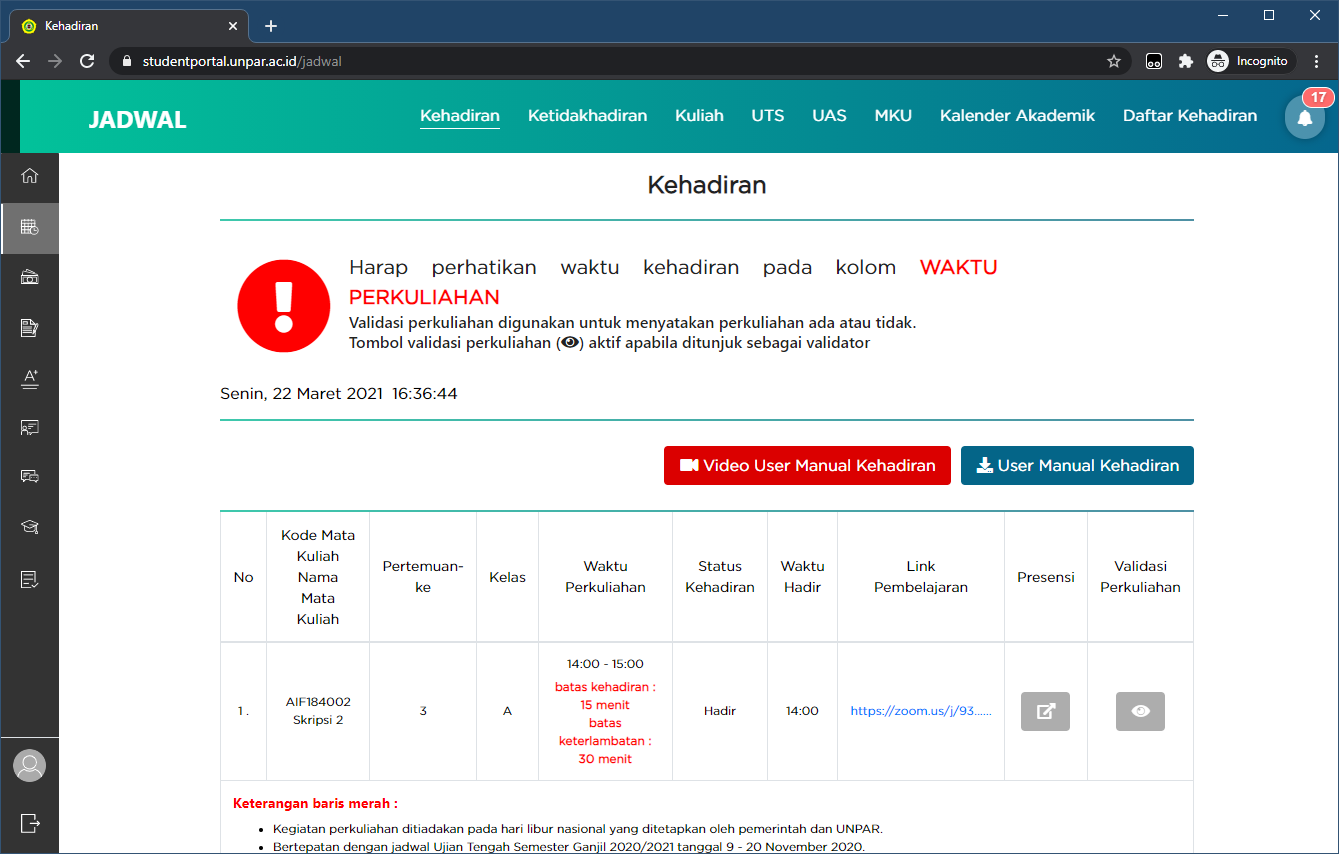
\includegraphics[scale=0.45]{Gambar/jadwal_kehadiran.png}
    			\caption{Halaman Kehadiran}
    			\label{fig:3_kehadiran}
			\end{figure}
			\item Ketidakhadiran\\
		    Submenu ini berfungsi untuk mengunggah surat sakit atau surat izin mahasiswa. (Gambar \ref{fig:3_ketidakhadiran}).
		    \begin{figure}[H]
    			\centering
    			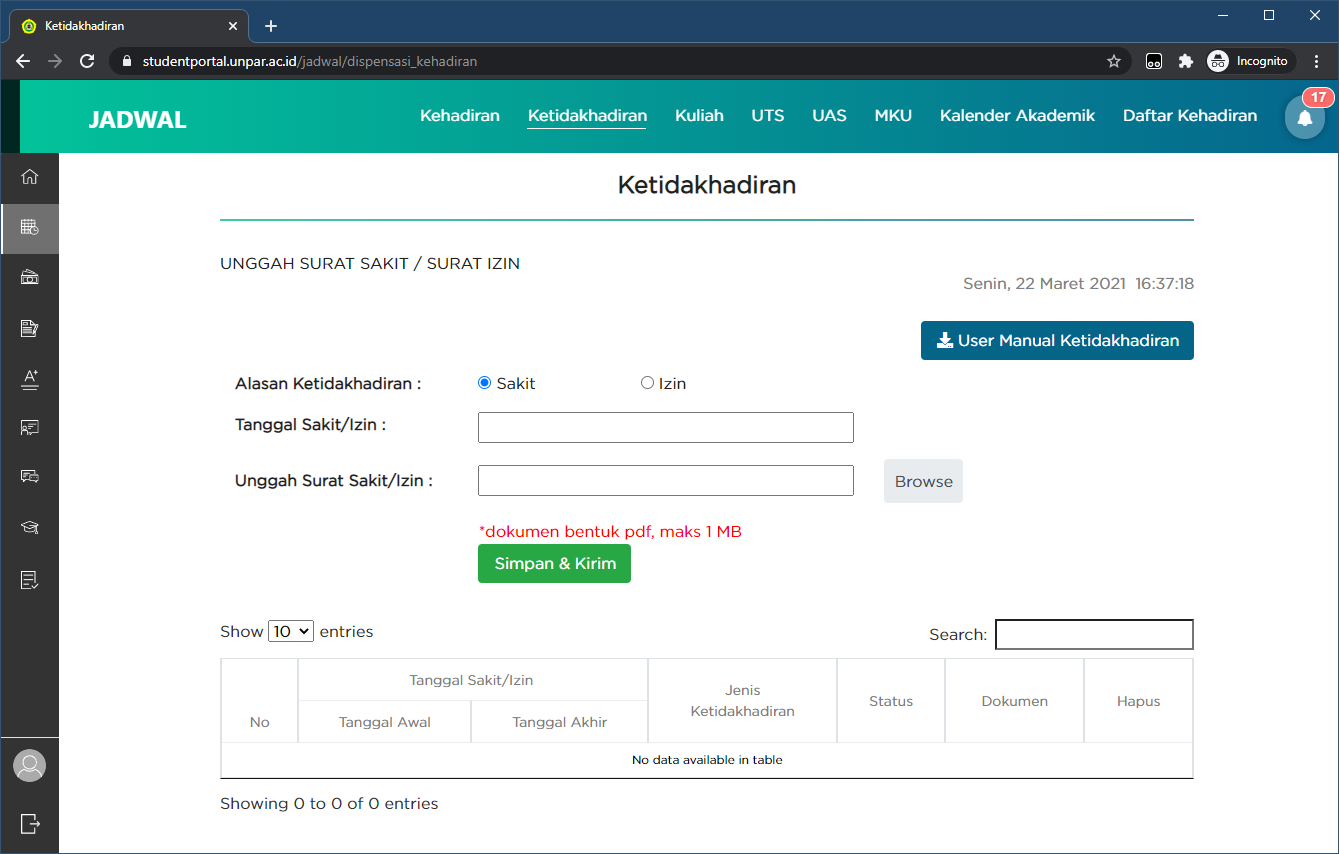
\includegraphics[scale=0.45]{Gambar/jadwal_ketidakhadiran.png}
    			\caption{Halaman Ketidakhadiran}
    			\label{fig:3_ketidakhadiran}
			\end{figure}
			\item Kuliah \\
			Submenu ini berisi tentang jadwal kuliah yang dapat disusun per semester dan terdapat 2 tampilan, yaitu tabel waktu (Gambar \ref{fig:3_jadwal_kuliah}) dan tabel biasa (Gambar \ref{fig:3_jadwal_kuliah_table}).
			\begin{figure}[H]
    			\centering
    			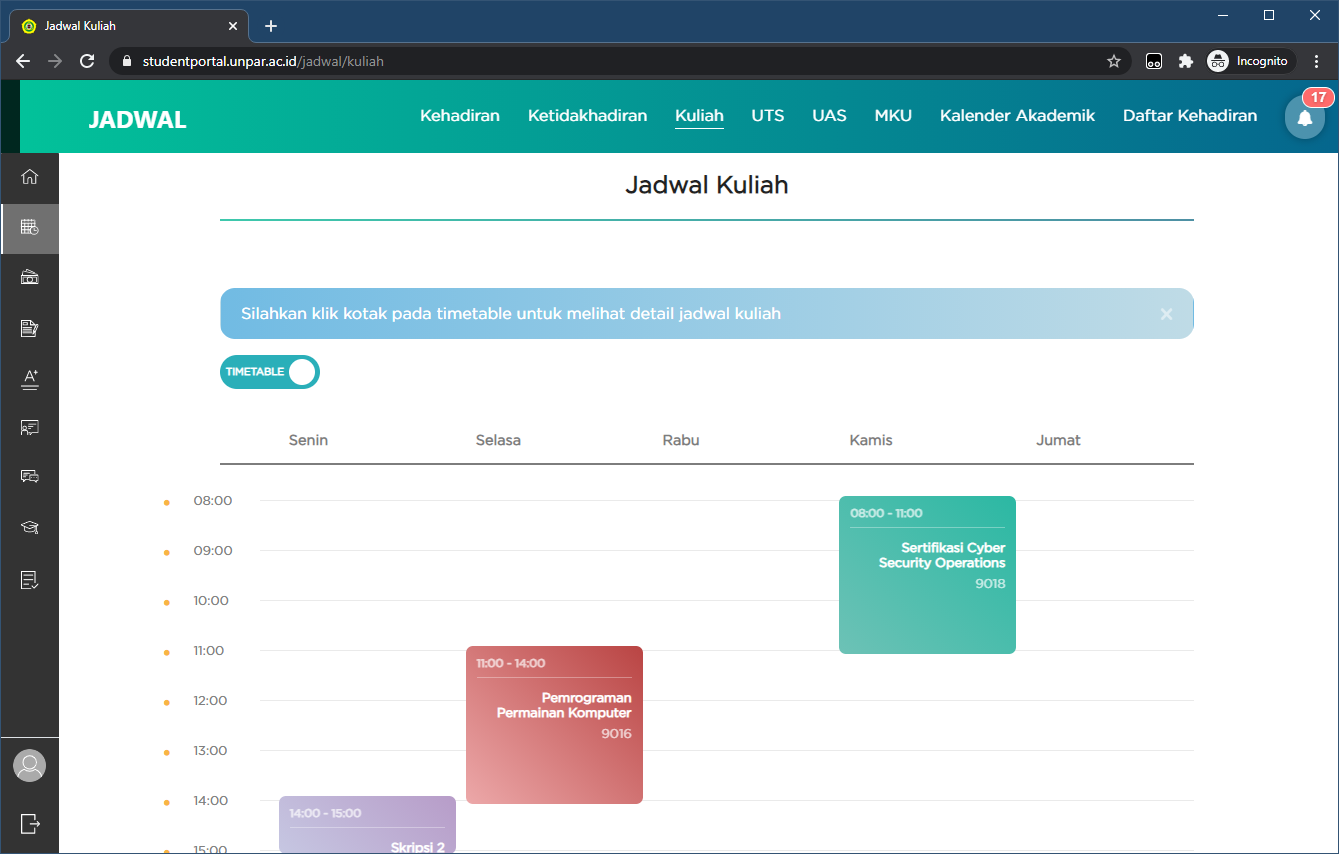
\includegraphics[scale=0.45]{Gambar/jadwal_kuliah.png}
    			\caption{Halaman Jadwal Kuliah Dalam Tabel Waktu}
    			\label{fig:3_jadwal_kuliah}
			\end{figure}
			\begin{figure}[H]
    			\centering
    			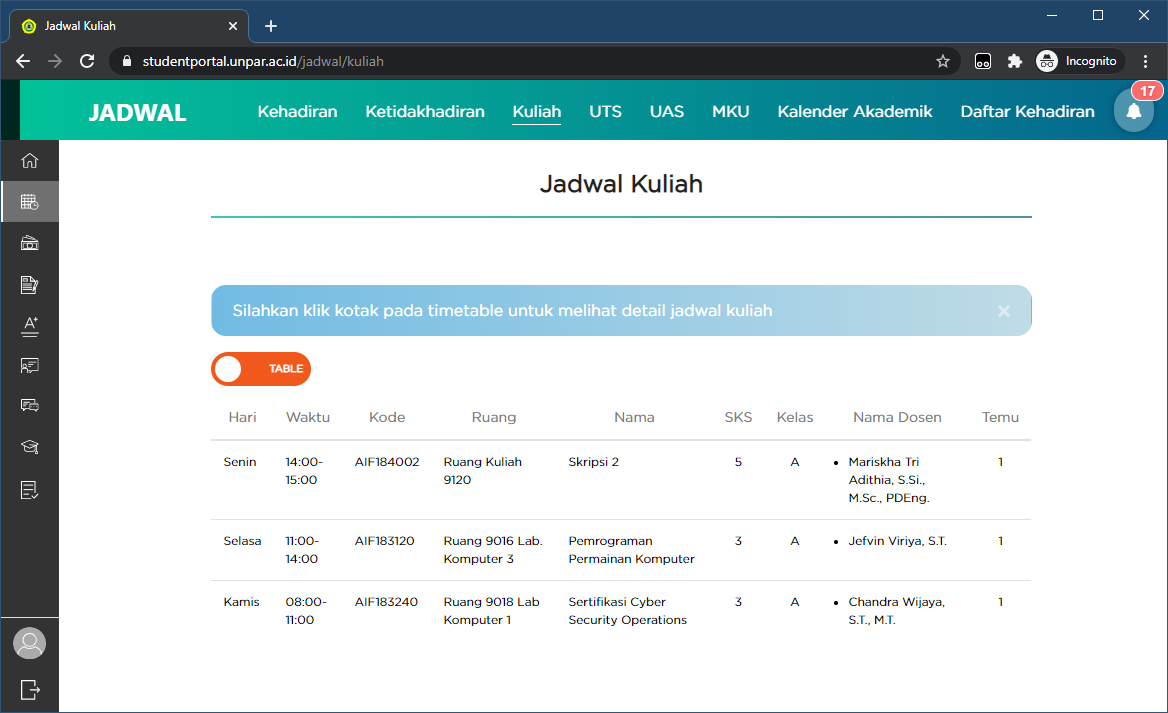
\includegraphics[scale=0.45]{Gambar/jadwal_kuliah_table.png}
    			\caption{Halaman Jadwal Kuliah Tabel}
    			\label{fig:3_jadwal_kuliah_table}
			\end{figure}
			\item UTS \\
			Submenu ini berisi tentang UTS yang dapat disusun per semester (Gambar \ref{fig:3_uts}).
			\begin{figure}[H]
    			\centering
    			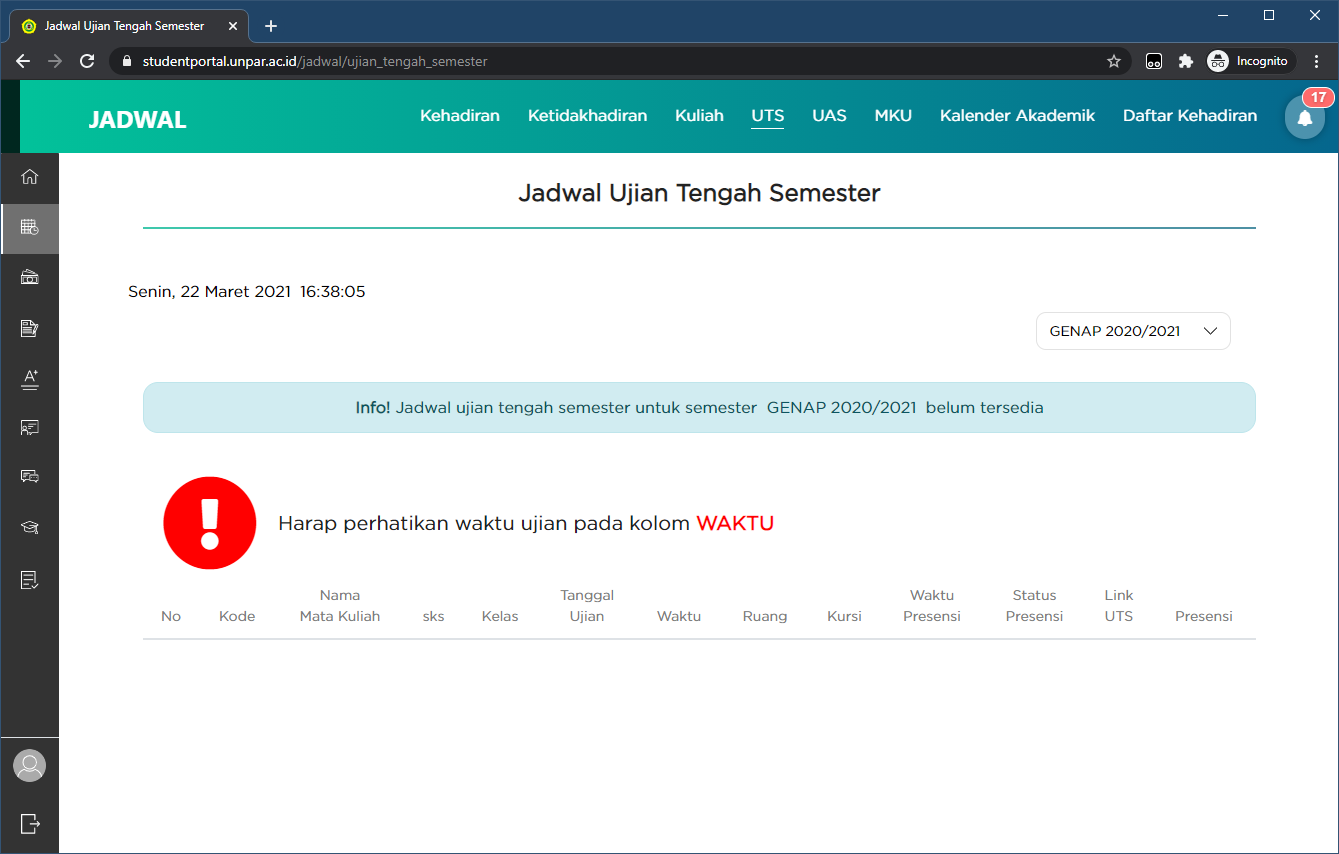
\includegraphics[scale=0.45]{Gambar/jadwal_uts.png}
    			\caption{Halaman UTS}
    			\label{fig:3_uts}
			\end{figure}
			\item UAS \\
			Submenu ini berisi tentang UAS yang dapat disusun per semester (Gambar \ref{fig:3_uas}).
			\begin{figure}[H]
    			\centering
    			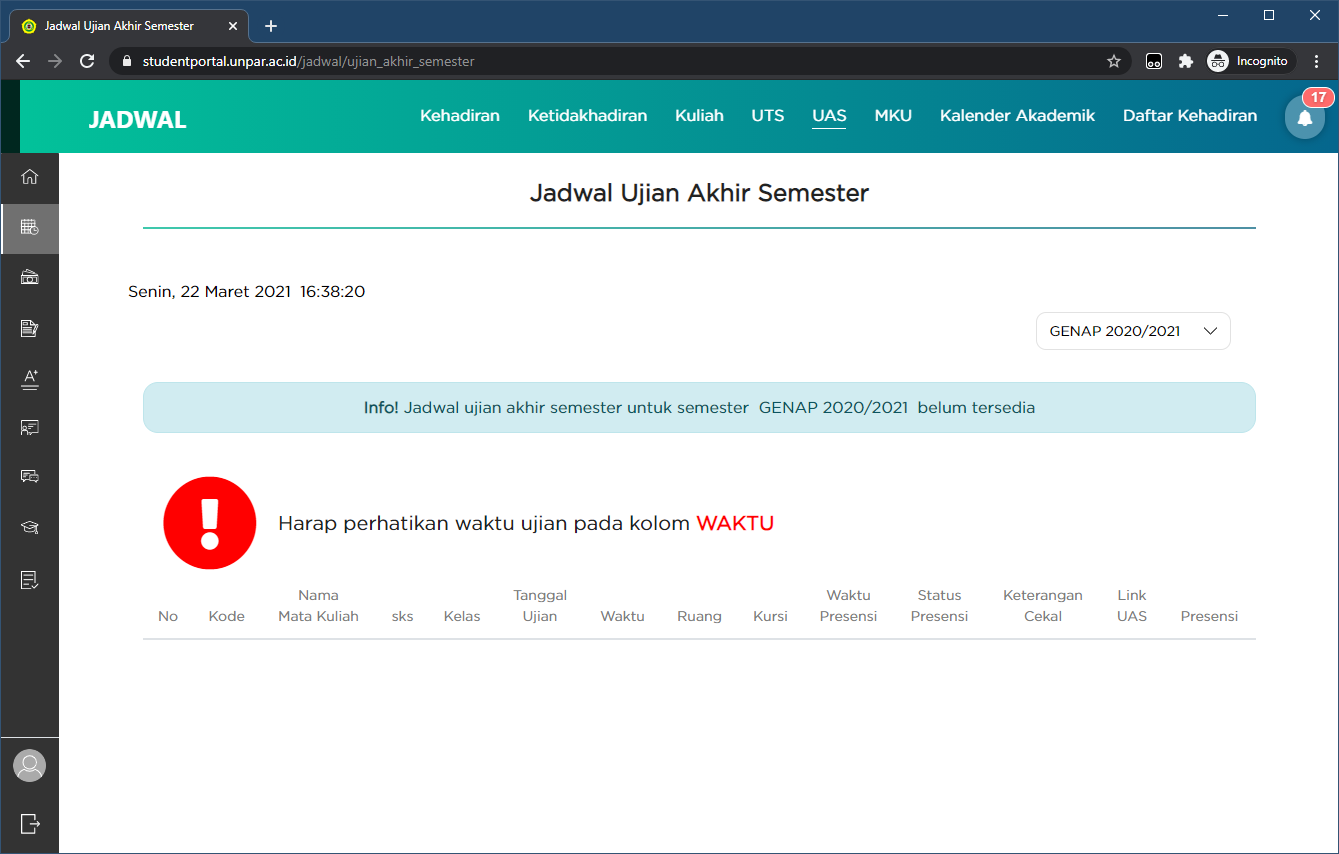
\includegraphics[scale=0.45]{Gambar/jadwal_uas.png}
    			\caption{Halaman UAS}
    			\label{fig:3_uas}
			\end{figure}
			\item MKU \\
			Submenu ini menampilkan seluruh jadwal Mata Kuliah Umum (MKU) yang memberikan informasi tentang kelas-kelas yang dibuka oleh Pusat Kajian Humaniora (PKH) (Gambar \ref{fig:3_mku}).
			\begin{figure}[H]
    			\centering
    			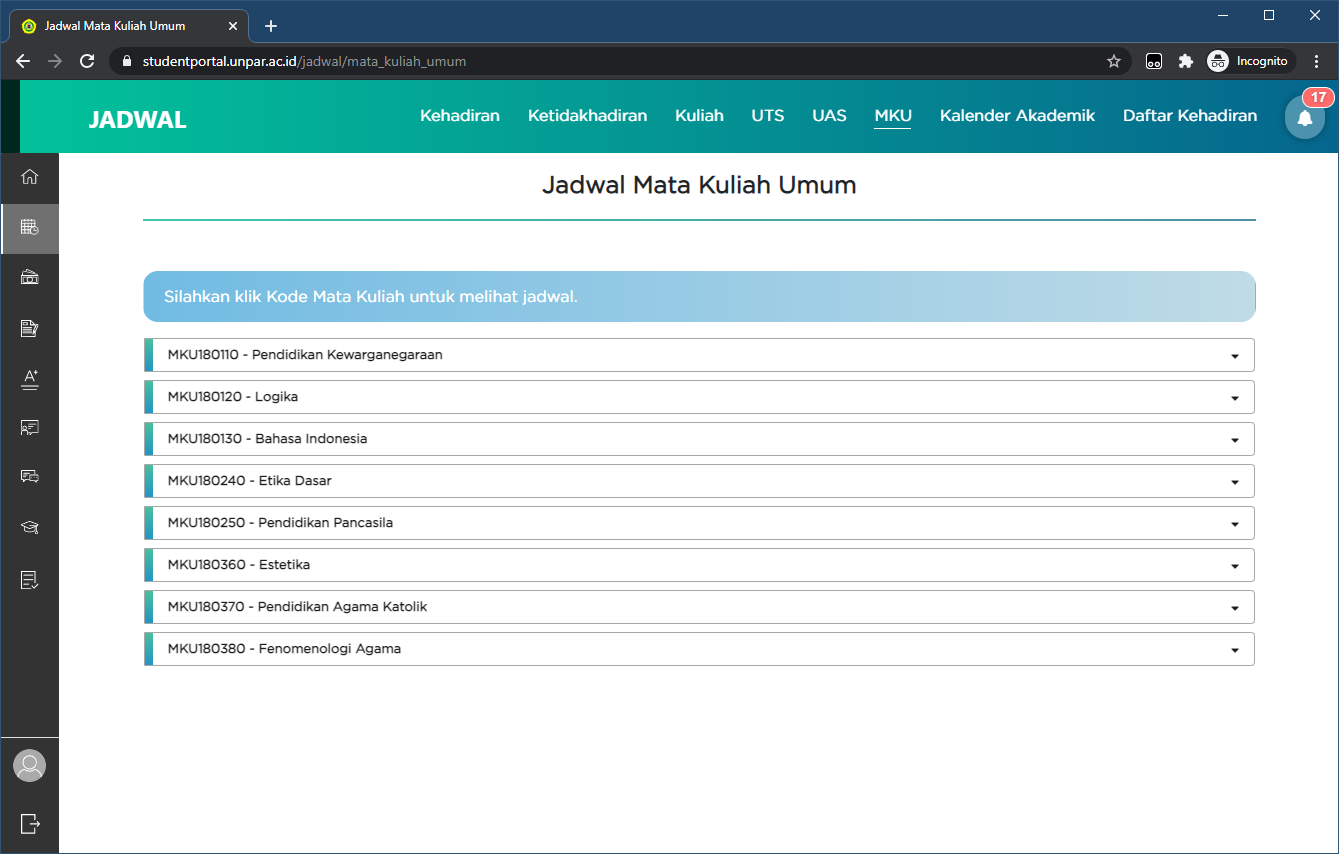
\includegraphics[scale=0.45]{Gambar/jadwal_mku.png}
    			\caption{Halaman MKU}
    			\label{fig:3_mku}
			\end{figure}
			\item Kalender Akademik \\
			Submenu ini menampilkan informasi mengenai kalender akademik UNPAR (Gambar \ref{fig:3_kalender_akademik}).
			\begin{figure}[H]
    			\centering
    			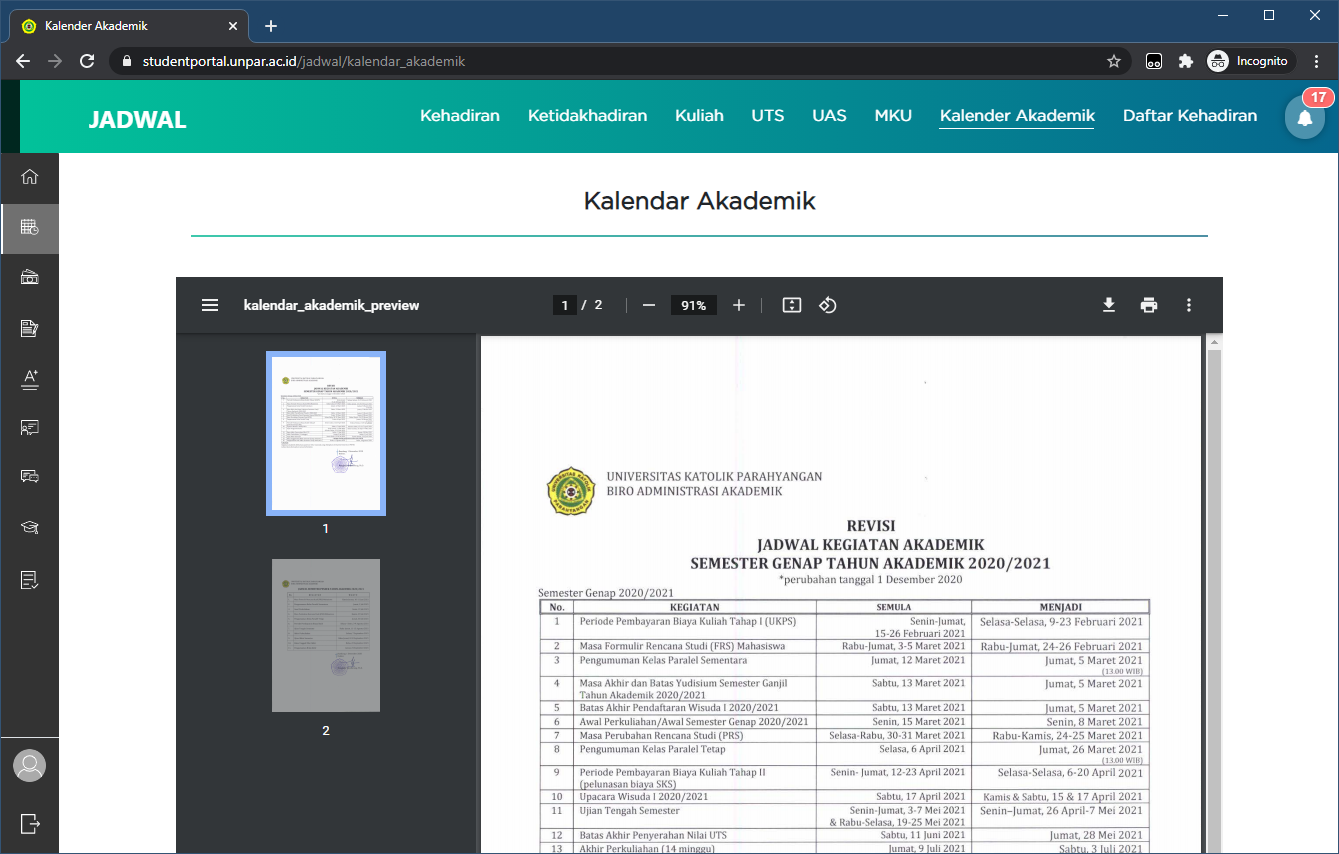
\includegraphics[scale=0.45]{Gambar/jadwal_kalenderakademik.png}
    			\caption{Halaman Kalender Akademik}
    			\label{fig:3_kalender_akademik}
			\end{figure}
			\item Daftar Kehadiran \\
			Submenu ini menampilkan informasi mengenai daftar kehadiran mahasiswa pada setiap mata kuliah yang dapat disusun per semester (Gambar \ref{fig:3_daftar_kehadiran}).
			\begin{figure}[H]
    			\centering
    			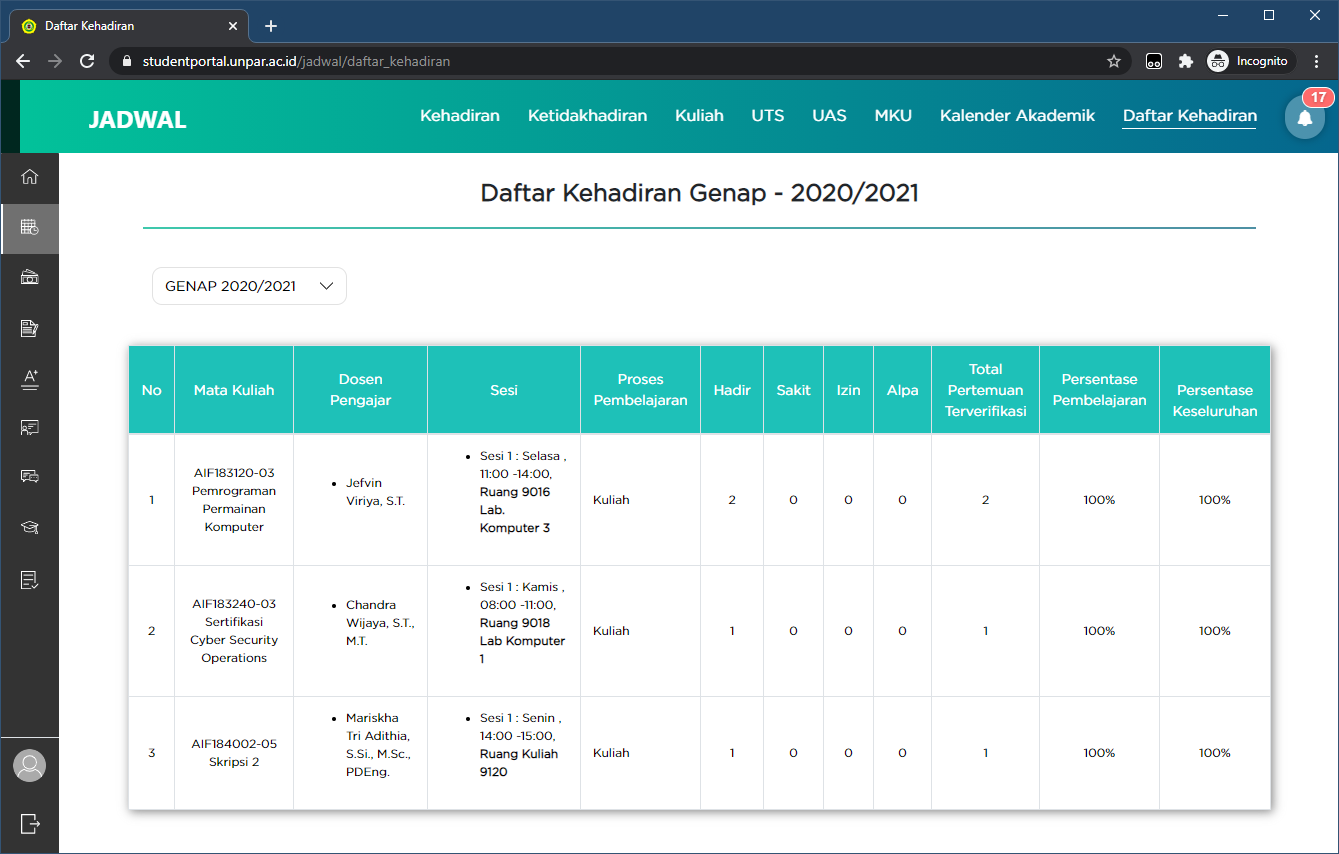
\includegraphics[scale=0.45]{Gambar/jadwal_daftarkehadiran.png}
    			\caption{Halaman Daftar Kehadiran}
    			\label{fig:3_daftar_kehadiran}
			\end{figure}
		\end{itemize}
    
\subsection{Pembayaran}
    Menu ini berfungsi untuk melihat data tagihan pembayaran uang kuliah, riwayat pembayaran, dan keterangan cara-cara pembayaran uang kuliah yang dapat disusun per semester (Gambar \ref{fig:3_pembayaran}).
	\begin{figure}[H]
		\centering
		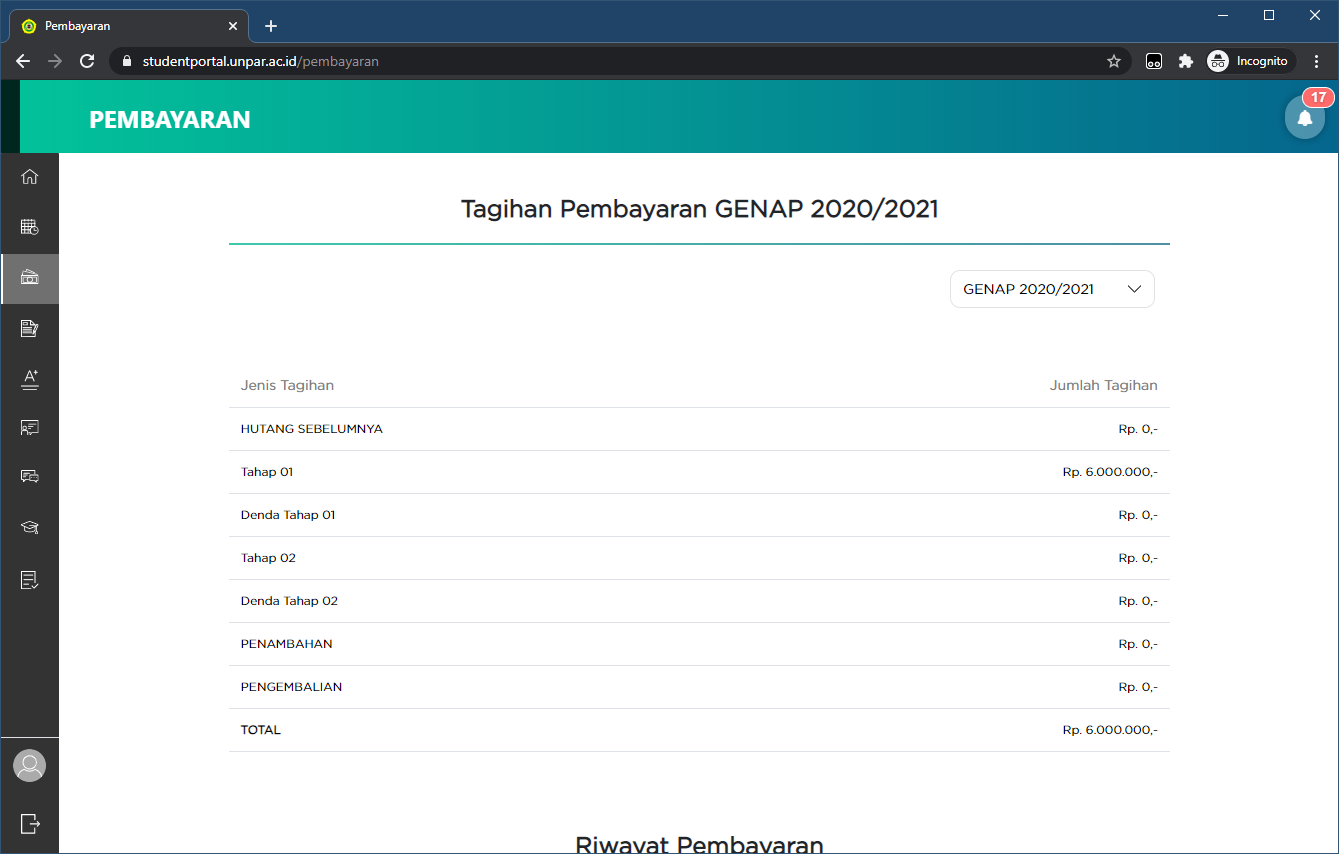
\includegraphics[scale=0.45]{Gambar/pembayaran.png}
		\caption{Halaman Pembayaran}
		\label{fig:3_pembayaran}
	\end{figure}  

\subsection{FRS/PRS}
    Menu ini berfungsi sebagai formulir pengisian rencana studi awal (FRS), perubahan rencana studi (PRS) dan menampilkan informasi mata kuliah yang telah diambil saat FRS atau PRS (Gambar \ref{fig:3_frs}).
	\begin{figure}[H]
		\centering
		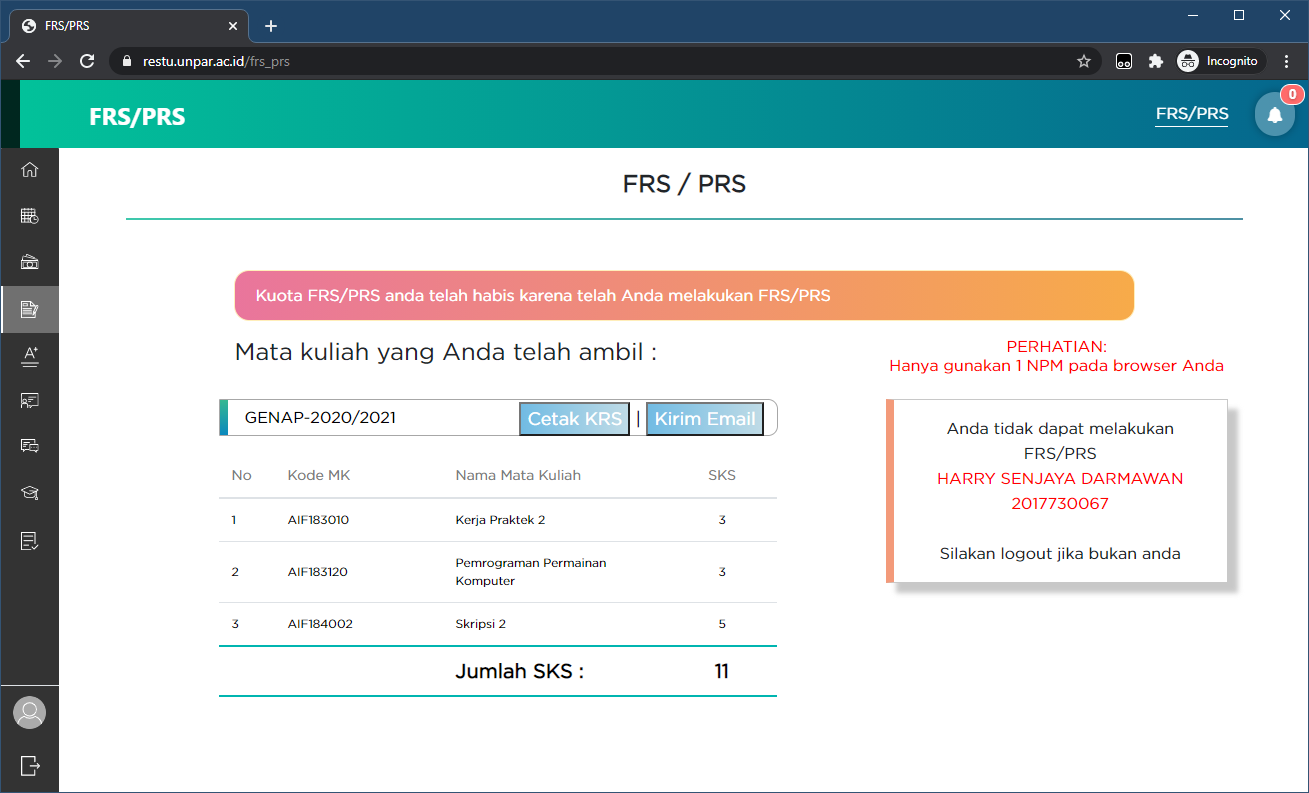
\includegraphics[scale=0.45]{Gambar/frs.png}
		\caption{Tampilan FRS/PRS}
		\label{fig:3_frs}
	\end{figure}
			

\subsection{Nilai}
    Menu Nilai terdiri dari beberapa submenu:
    
    \begin{itemize}
        \item Nilai per Semester\\
        Submenu ini menampilkan informasi nilai per semester. Mahasiswa dapat melihat nilai sesuai dengan semester yang dipilih (Gambar \ref{fig:3_nilai_per_semester}). 
        % Semester yang sedang diambil oleh mahasiswa dapat digunakan untuk ditampilkan pada \textit{screensaver}. Pengambilan semester tersebut dilakukan dengan mencari elemen dengan nama "dropdownSemester". 
        
        \begin{figure}[H]
        	\centering
        	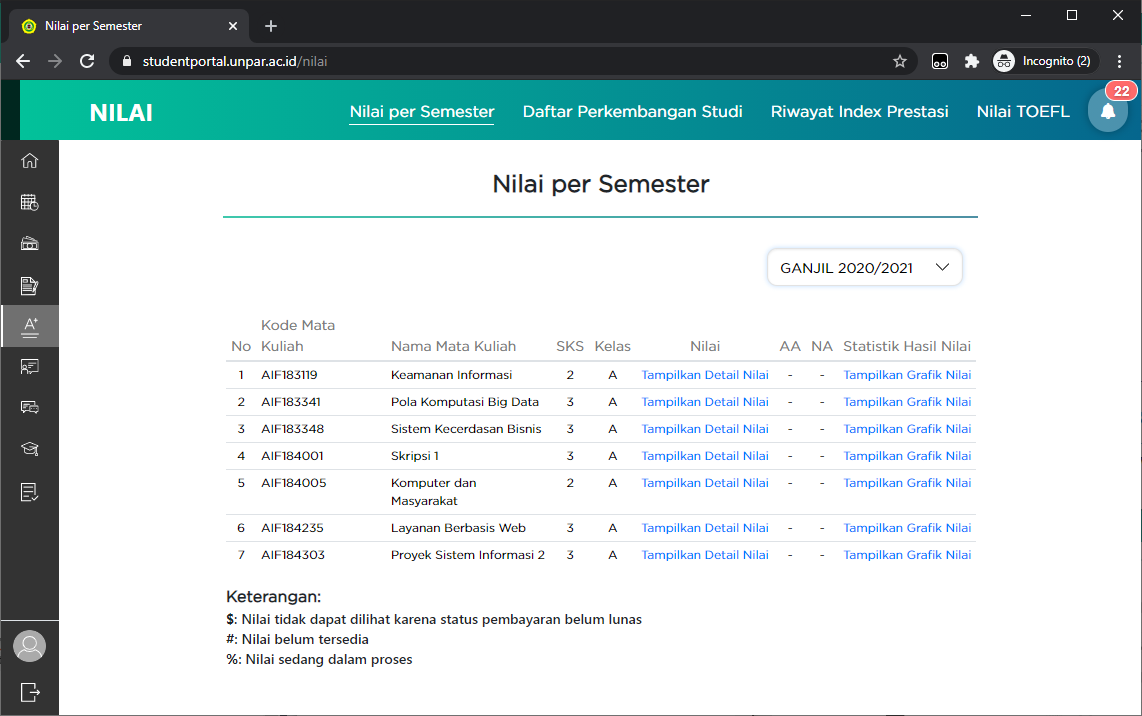
\includegraphics[scale=0.45]{Gambar/nilai_per_semester.png}
        	\caption{Halaman Nilai Per Semester} 
        	\label{fig:3_nilai_per_semester}
        \end{figure}
        
        \item Daftar Perkembangan Studi\\
        Submenu ini menampilkan seluruh riwayat mata kuliah dan nilai yang pernah ditempuh mahasiswa (Gambar \ref{fig:3_dps_1}). Submenu ini juga menampilkan statistik sks, nilai, dan indeks prestasi mahasiswa (Gambar \ref{fig:3_dps_2}).
        \begin{figure}[H]
        	\centering
        	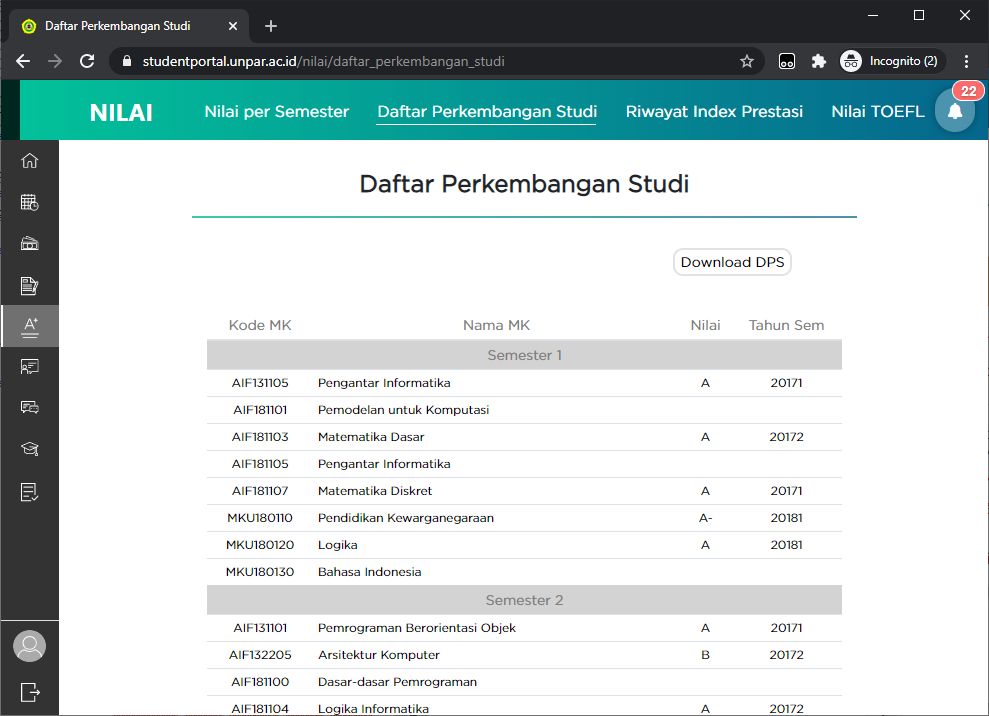
\includegraphics[scale=0.45]{Gambar/nilai_dps_1.png}
        	\caption{Halaman Daftar Perkembangan Studi (1)} 
        	\label{fig:3_dps_1}
        \end{figure}
        
         \begin{figure}[H]
        	\centering
        	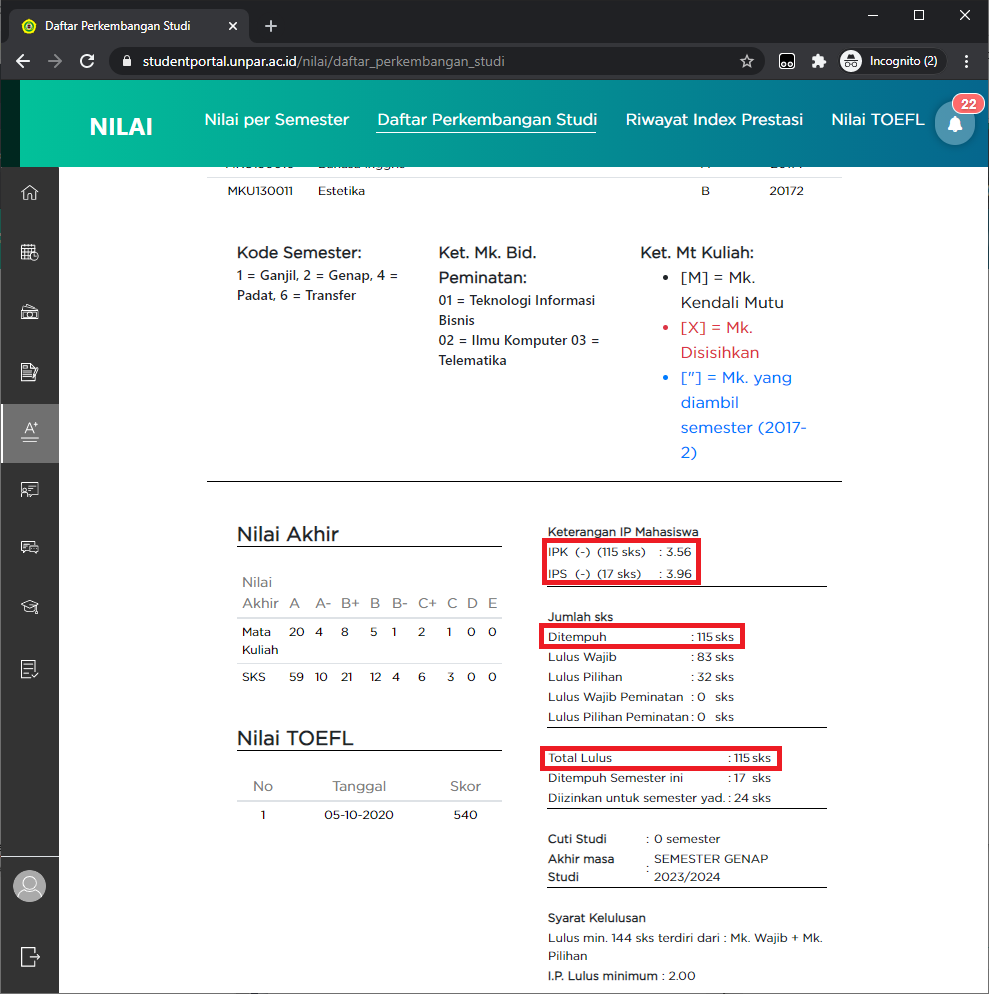
\includegraphics[scale=0.45]{Gambar/nilai_dps_2.png}
        	\caption{Halaman Daftar Perkembangan Studi (2)} 
        	\label{fig:3_dps_2}
        \end{figure}
        
        \item Riwayat Indeks Prestasi\\
       Submenu ini menampilkan seluruh riwayat Indeks Prestasi Semester (IPS) dan Indeks Prestasi Kumulatif (IPK) setiap semester mahasiswa (Gambar \ref{fig:3_rip}).
       
       \begin{figure}[H]
        	\centering
        	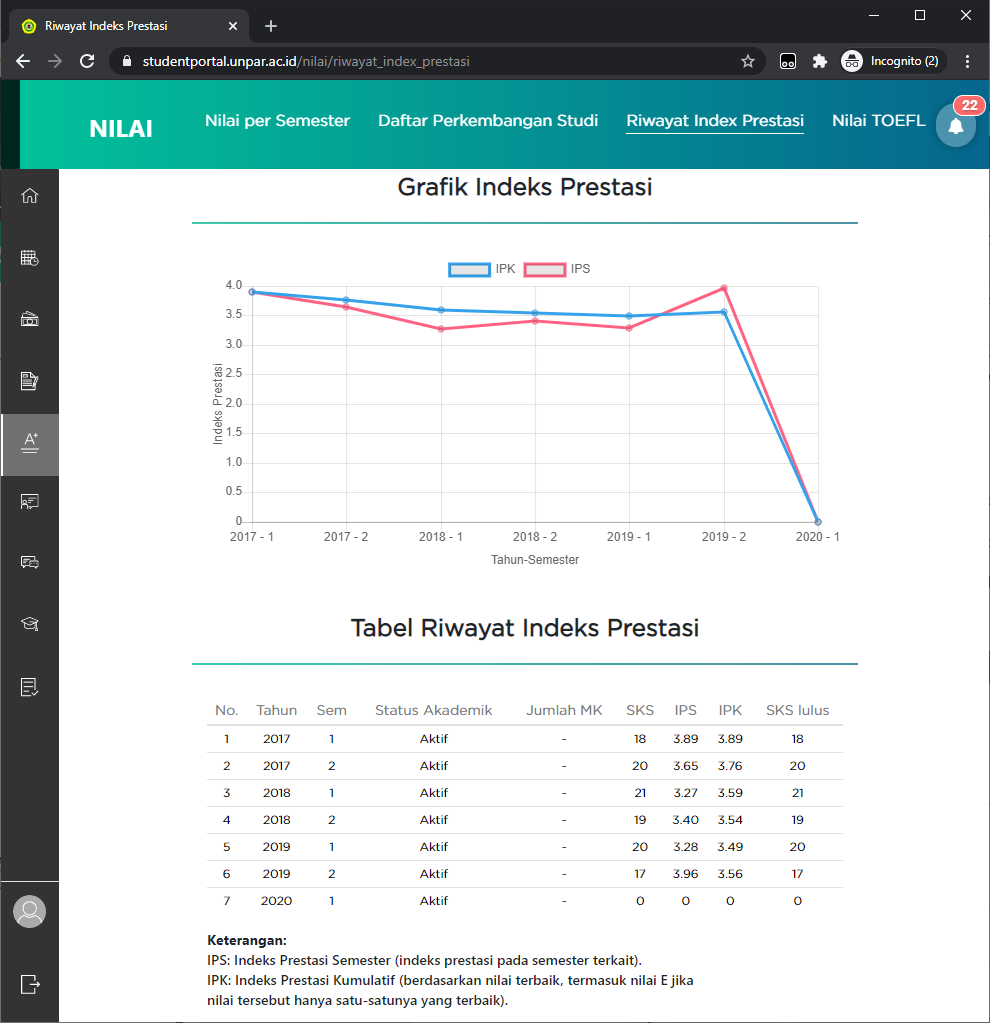
\includegraphics[scale=0.45]{Gambar/nilai_rip.png}
        	\caption{Halaman Riwayat Indeks Prestasi} 
        	\label{fig:3_rip}
        \end{figure}
        
        \item Nilai TOEFL\\
       Submenu ini menampilkan seluruh riwayat skor dan detail skor \textit{Test of English as Foreign Language} (TOEFL) yang pernah ditempuh mahasiswa (Gambar \ref{fig:3_toefl}). 

        \begin{figure}[H]
        	\centering
        	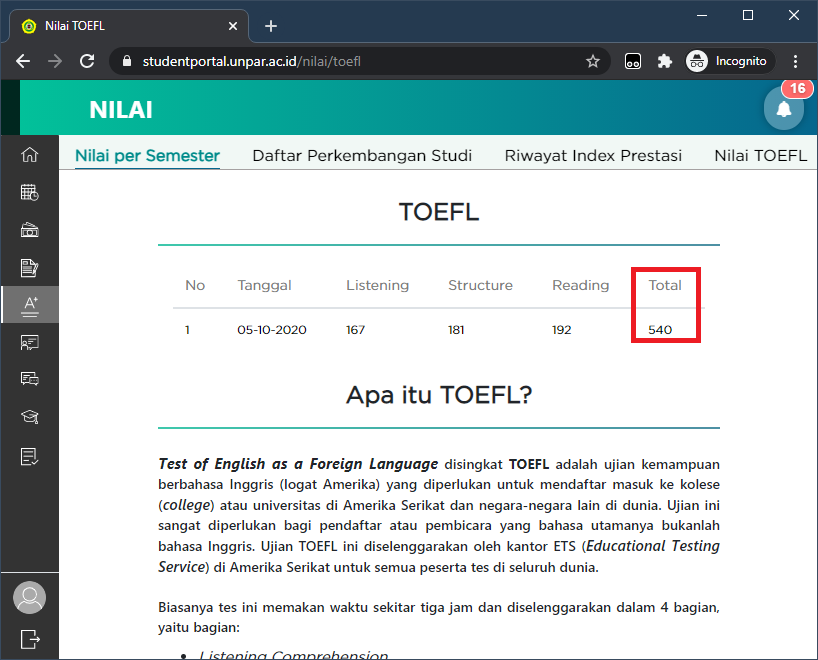
\includegraphics[scale=0.45]{Gambar/nilai_toefl.png}
        	\caption{Halaman Nilai TOEFL} 
        	\label{fig:3_toefl}
        \end{figure}

    \end{itemize}
    
\subsection{Angket}
    Menu Angket merupakan halaman dimana mahasiswa diminta untuk mengisi angket dari para dosen yang mengajarnya di semester yang sedang ditempuh mahasiswa tersebut (Gambar \ref{fig:3_angket}).
        \begin{figure}[H]
        	\centering
        	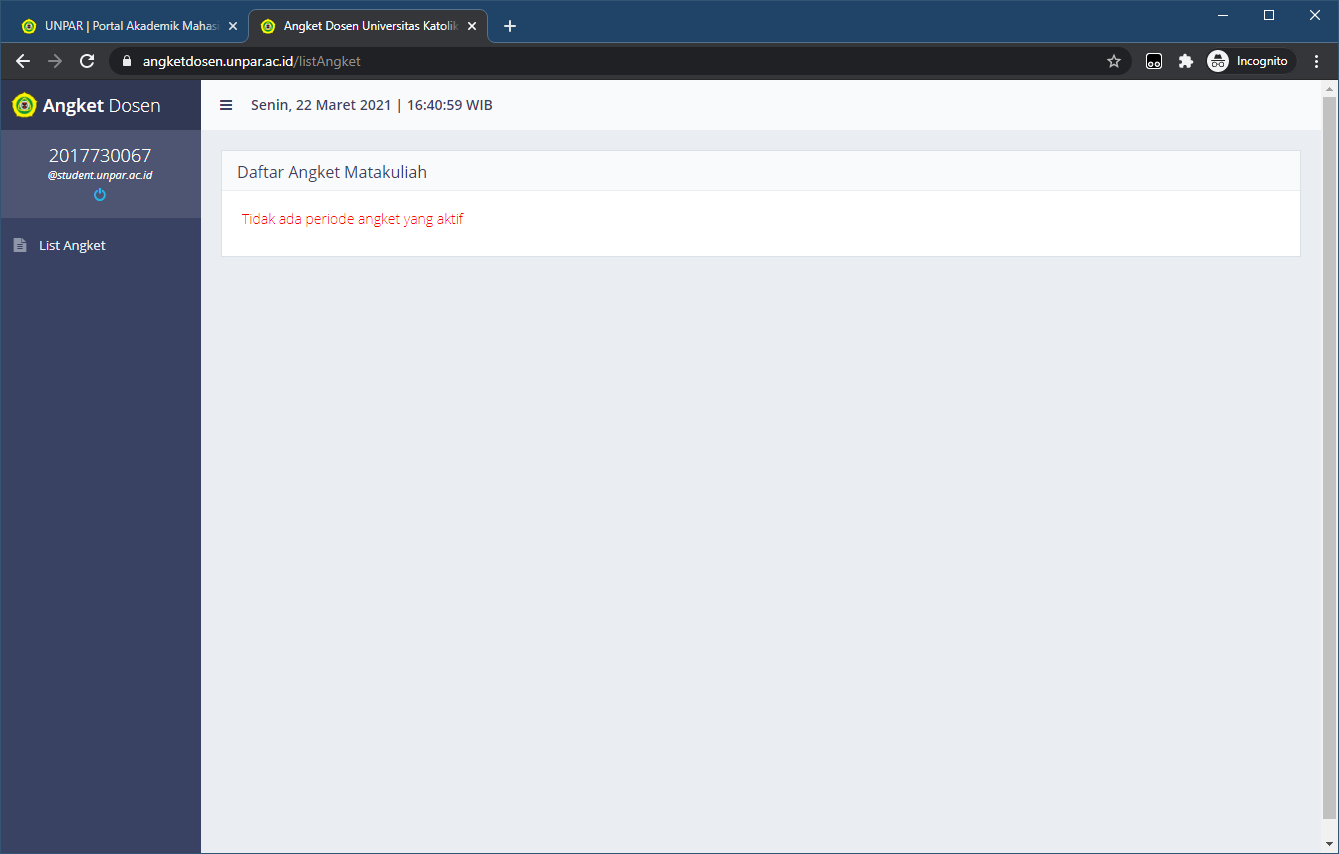
\includegraphics[scale=0.45]{Gambar/angket.png}
        	\caption{Halaman Angket} 
        	\label{fig:3_angket}
        \end{figure}
        
\subsection{Saran \& Komentar}
    Menu Saran \& Komentar akan membuka halaman \url{https://suaramahasiswa.unpar.ac.id/} (Gambar \ref{fig:3_saran_komentar}).
    \begin{figure}[H]
    	\centering
    	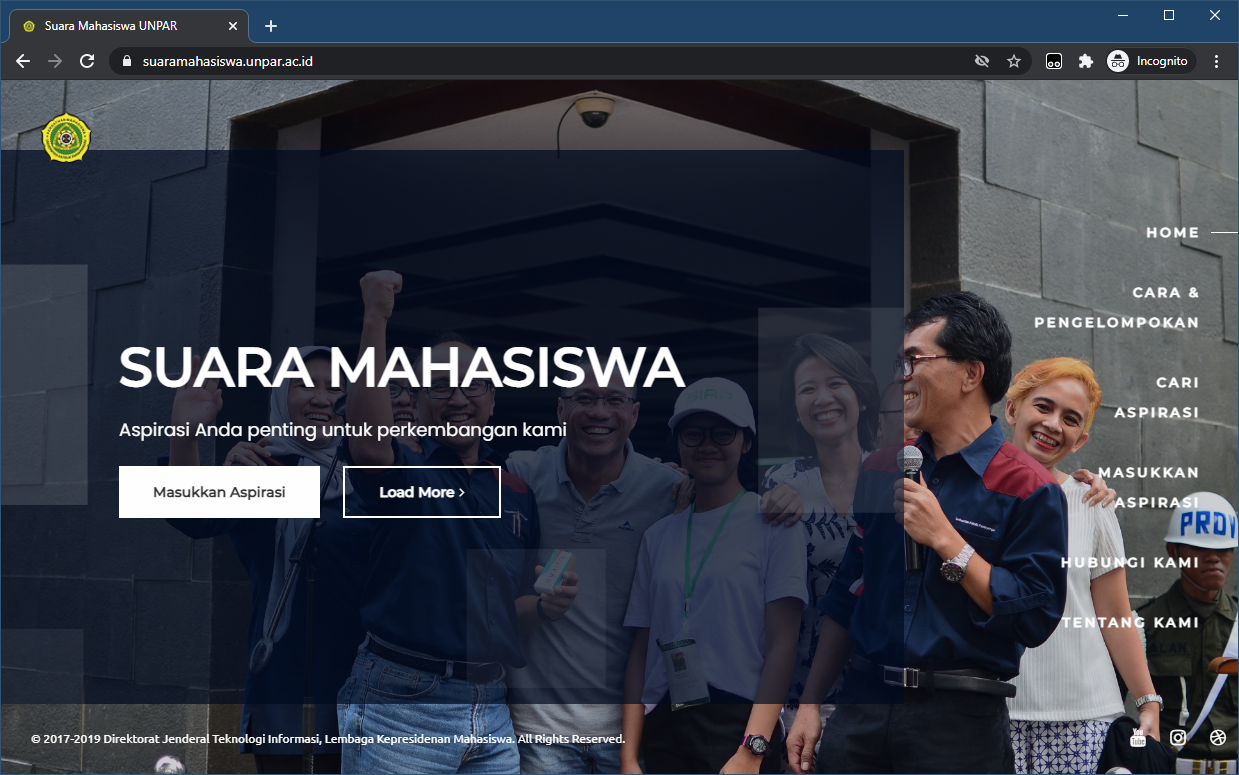
\includegraphics[scale=0.45]{Gambar/sarankomentar.png}
    	\caption{Halaman Saran \& Komentar} 
    	\label{fig:3_saran_komentar}
    \end{figure}
        
\subsection{Kelulusan}
    Menu Kelulusan sedang dalam tahap pembangunan (Gambar \ref{fig:3_kelulusan}).
    \begin{figure}[H]
    	\centering
    	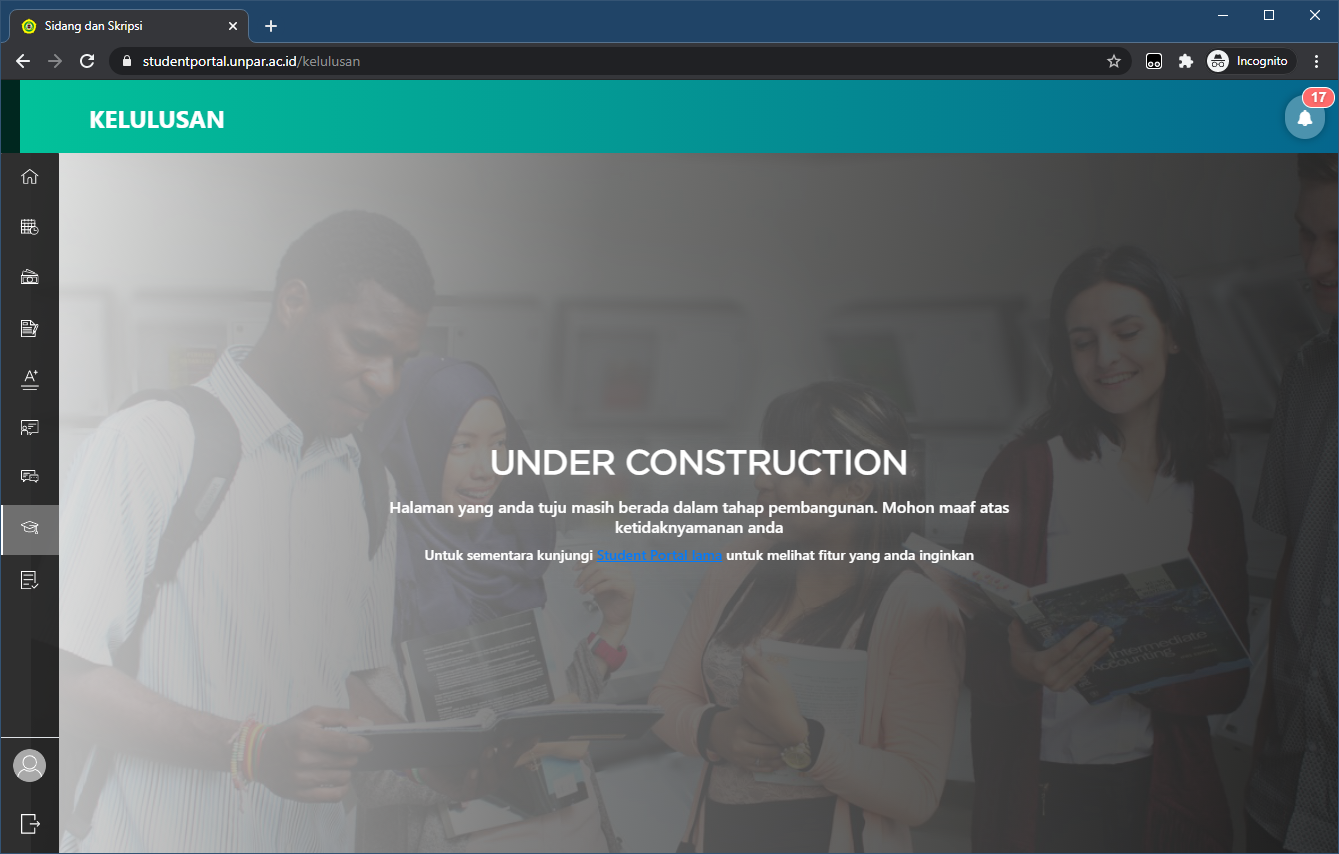
\includegraphics[scale=0.45]{Gambar/kelulusan.png}
    	\caption{Halaman Kelulusan} 
    	\label{fig:3_kelulusan}
    \end{figure}

\subsection{Pengajuan}
    Menu Pengajuan merupakan halaman dimana mahasiswa dapat mengajukan topik skripsi atau tugas akhir (Gambar \ref{fig:3_pengajuan}).
    \begin{figure}[H]
    	\centering
    	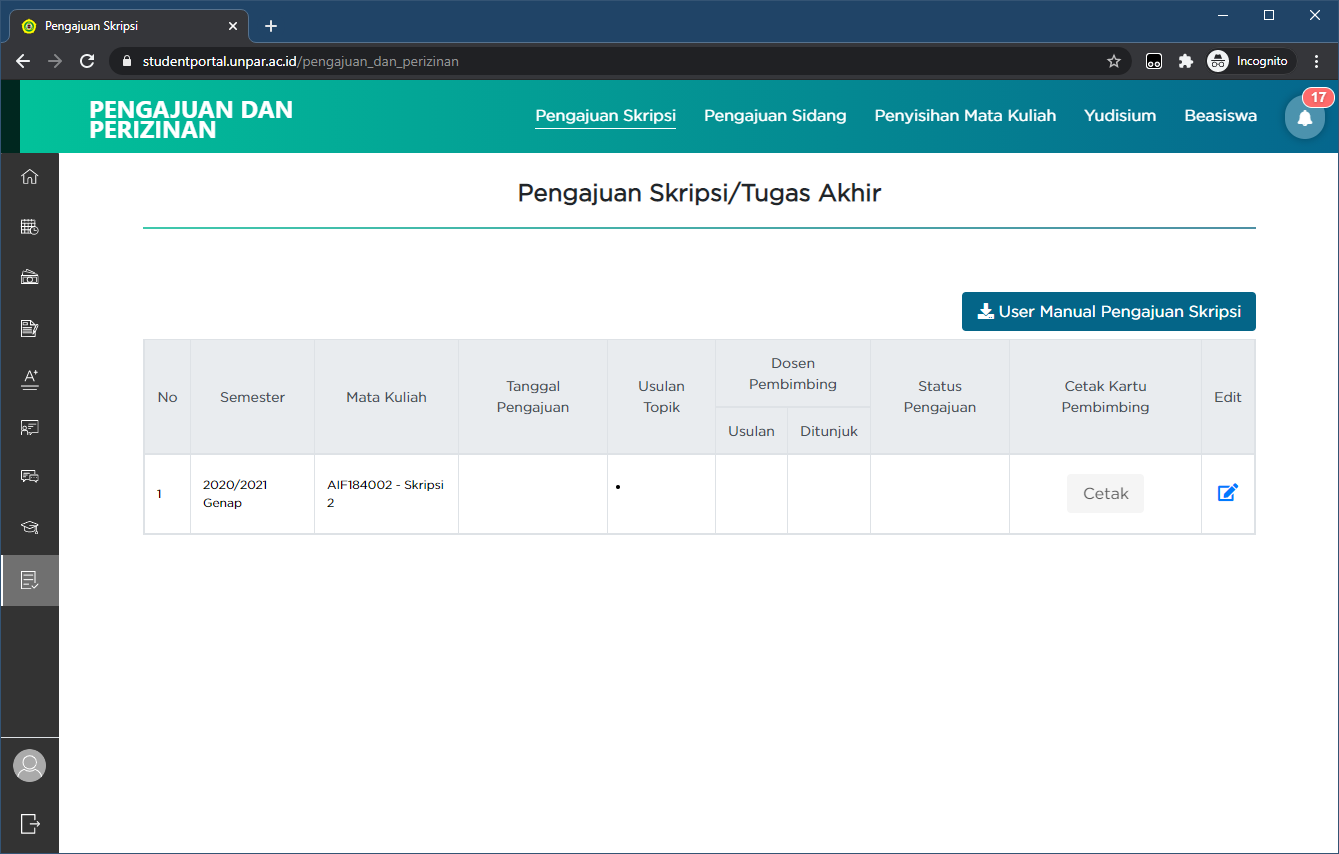
\includegraphics[scale=0.45]{Gambar/pengajuan.png}
    	\caption{Halaman Pengajuan} 
    	\label{fig:3_pengajuan}
    \end{figure}
    
    
\section{Analisis SIAKAD}

\textit{Subbab ini ditulis oleh dosen pembimbing.}

SIAKAD adalah sistem informasi yang disediakan oleh Biro Teknologi Informasi kepada staf UNPAR, untuk menangani hal-hal yang berkaitan dengan akademik. SIAKAD dapat diakses pada alamat \url{https://siakad.unpar.ac.id} dari lingkungan jaringan UNPAR atau melalui VPN (\textit{Virtual Private Network}). Modul-modul yang ditampilkan pada SIAKAD dapat berbeda, bergantung pada peran pengguna yang login. Pada subbab ini, akan dijabarkan modul-modul yang ditampilkan kepada dosen.

\subsection{Login}

Tata cara login untuk mengakses SIAKAD tidak jauh berbeda dengan pada Portal Akademik Mahasiswa. Dosen atau staf diarahkan ke situs web SSO (Gambar \ref{fig:3_login} dan \ref{fig:3_login_2}). Perbedaannya hanyalah bahwa SIAKAD membatasi hanya akun dosen atau staf yang diperbolehkan masuk, berdasarkan alamat e-mailnya.

\subsection{Mahasiswa}

Untuk dosen, hanya ada satu submenu dari menu Mahasiswa, yaitu ``Cari Mahasiswa''. Halaman ini memungkinkan dosen untuk mendapatkan daftar mahasiswa walinya. Untuk setiap mahasiswa, ada tiga tautan yang dapat diklik, yaitu: NPM (untuk membuka pop-up Detail Mahasiswa), Data Diri, dan Data Akademik. Gambar \ref{fig:3_siakad_carimahasiswa} menunjukkan tampilan daftar mahasiswa wali dosen.

\begin{figure}[H]
    \centering
    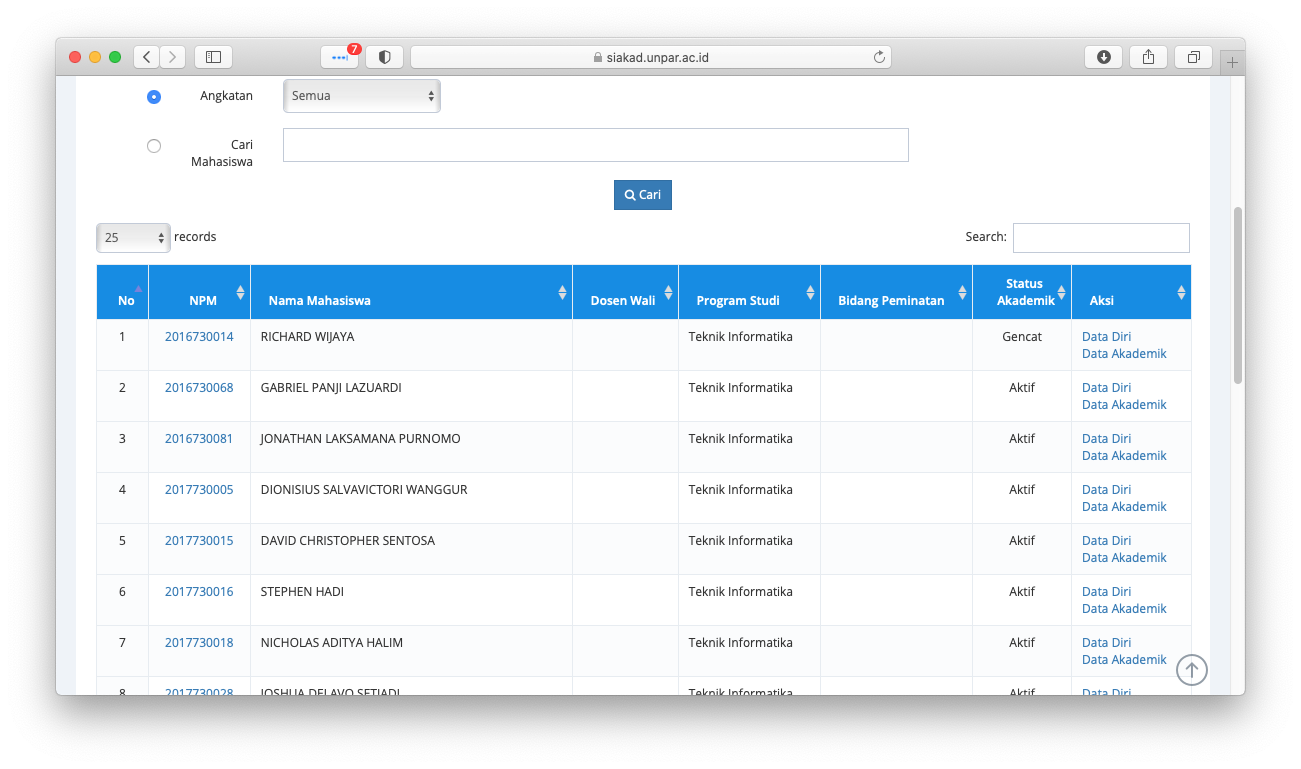
\includegraphics[scale=0.35]{Gambar/siakad_carimahasiswa.png}
    \caption{Tangkapan Layar Halaman Daftar Mahasiswa Wali}
    \label{fig:3_siakad_carimahasiswa}
\end{figure}

\paragraph{Detail Mahasiswa} Detail ringkas mahasiswa ditampilkan dalam bentuk pop-up (Gambar \ref{fig:3_siakad_detailmahasiswa}) sehingga dosen wali dapat melihat secara sekilas data mahasiswa satu per satu tanpa perlu berpindah ke halaman lain.

\begin{figure}[H]
    \centering
    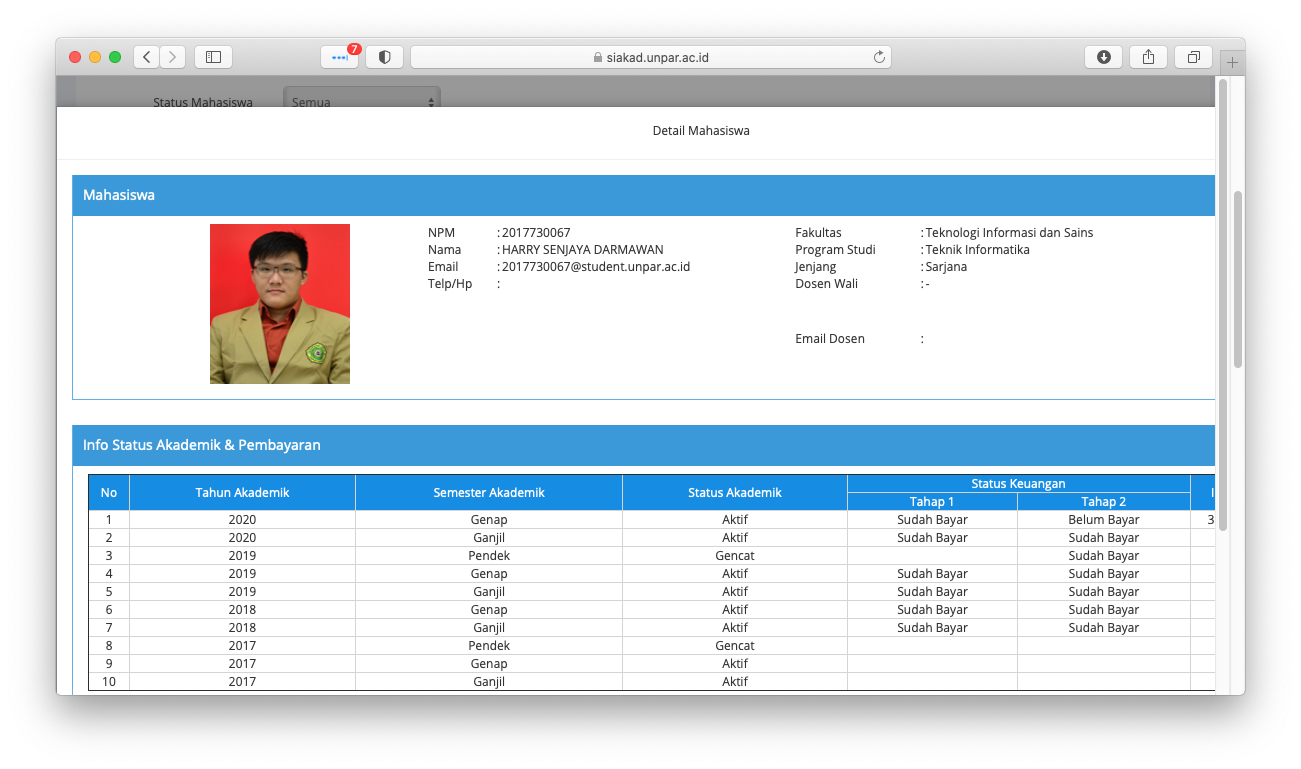
\includegraphics[scale=0.35]{Gambar/siakad_detailmahasiswa.png}
    \caption{Tangkapan Layar Pop-up Detail Mahasiswa}
    \label{fig:3_siakad_detailmahasiswa}
\end{figure}

\subsubsection{Data Diri}

Data diri mahasiswa ditampilkan pada halaman baru yang terdiri dari beberapa tab. Halaman ini berisi detail data diri / pribadi mahasiswa yang tidak terkait data akademik di UNPAR. Halaman ini terdiri dari tiga tab, yaitu Identitas Mahasiswa, Riwayat Pendidikan, dan Orang Tua/Wali.

\paragraph{Identitas Mahasiswa} Tab ini berisi data identitas mahasiswa, seperti foto, tempat/tanggal lahir, jenis kelamin, kewarganegaraan, serta data pribadi lainnya (Gambar \ref{fig:3_siakad_datadiri_identitasmahasiswa}).

\begin{figure}[H]
    \centering
    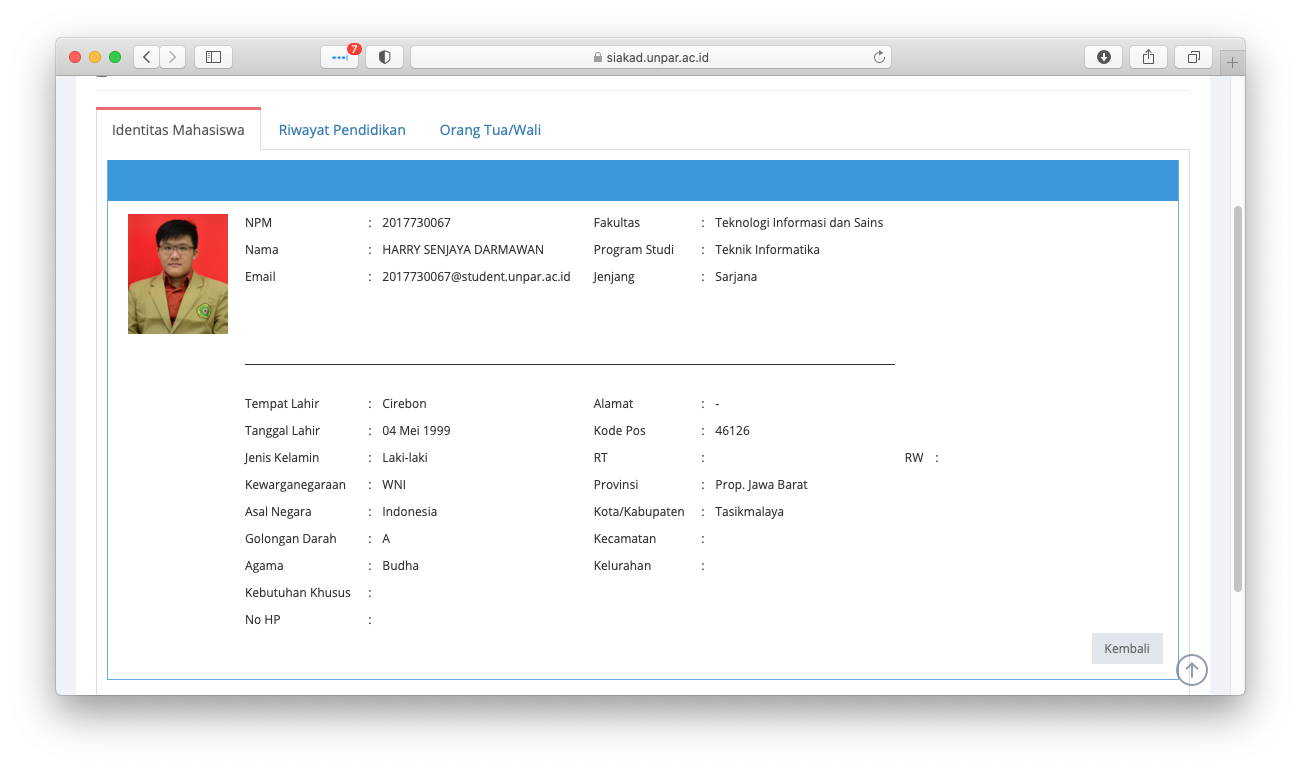
\includegraphics[scale=0.35]{Gambar/siakad_datadiri_identitasmahasiswa.png}
    \caption{Tangkapan Layar Tab Identitas Mahasiswa}
    \label{fig:3_siakad_datadiri_identitasmahasiswa}
\end{figure}

\paragraph{Riwayat Pendidikan} Tab ini berisi riwayat pendidikan mahasiswa sebelum berkuliah di UNPAR, baik SMA maupun di perguruan tinggi lain (Gambar \ref{fig:3_siakad_datadiri_riwayatpendidikan}).

\begin{figure}[H]
    \centering
    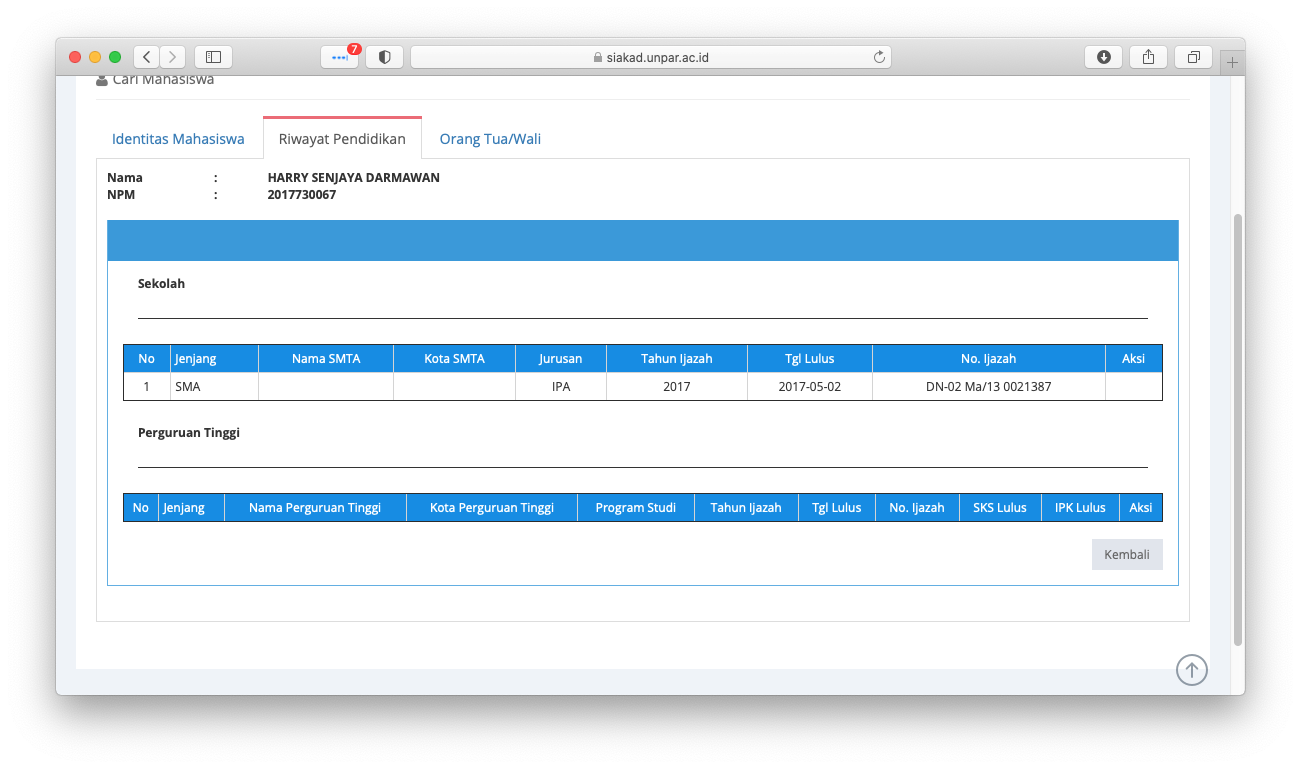
\includegraphics[scale=0.35]{Gambar/siakad_datadiri_riwayatpendidikan.png}
    \caption{Tangkapan Layar Tab Riwayat Pendidikan}
    \label{fig:3_siakad_datadiri_riwayatpendidikan}
\end{figure}

\paragraph{Orang Tua/Wali} Tab ini berisi data identitas orang tua atau wali mahasiswa, seperti nama, tempat/tanggal lahir, dan sebagainya (Gambar \ref{fig:3_siakad_datadiri_orangtuawali}).

\begin{figure}[H]
    \centering
    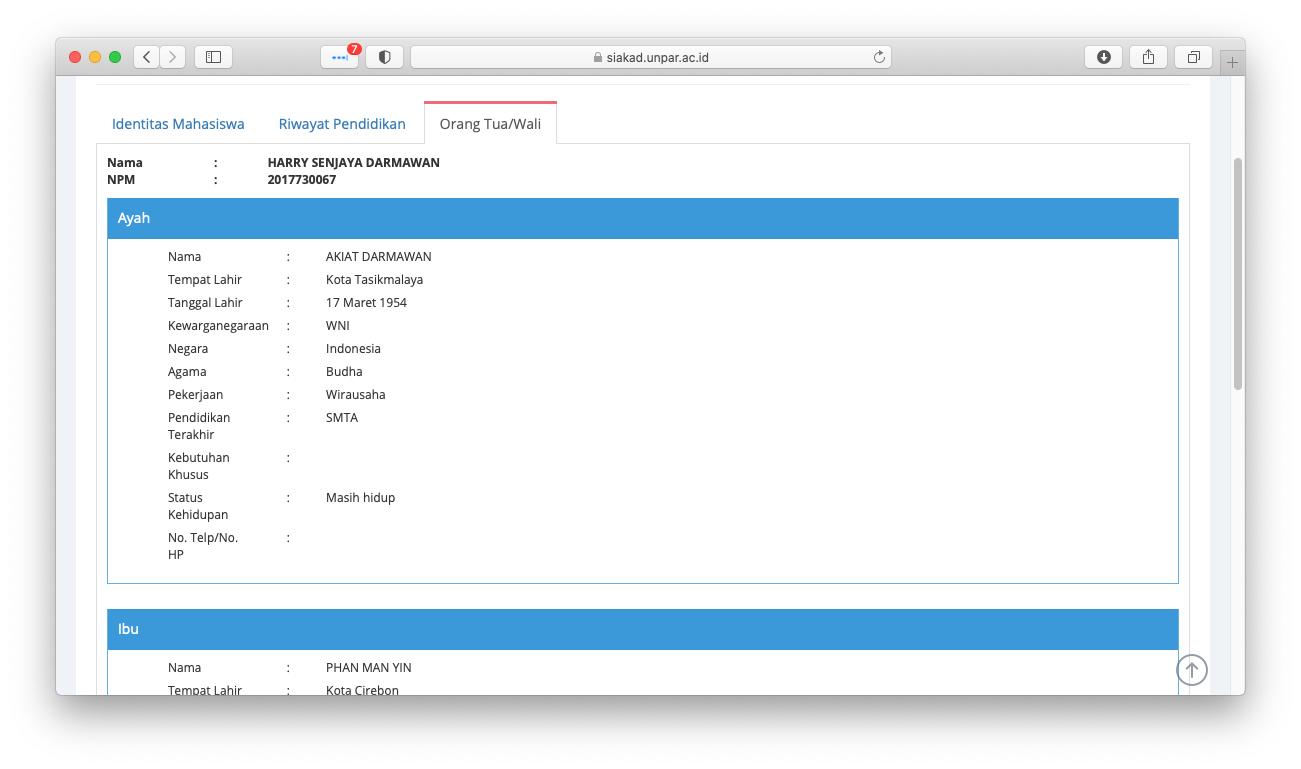
\includegraphics[scale=0.35]{Gambar/siakad_datadiri_orangtuawali.png}
    \caption{Tangkapan Layar Tab Orang Tua/Wali}
    \label{fig:3_siakad_datadiri_orangtuawali}
\end{figure}

\subsubsection{Data Akademik}

Data akademik mahasiswa ditampilkan pada halaman baru yang terdiri dari beberapa tab. Halaman ini berisi detail data akademik di UNPAR. Halaman ini terdiri dari lima tab, yaitu Ringkasan, Nilai Semester Ini, Nilai Per Tahun Semester, Nilai Berdasarkan Kurikulum, dan Status Akademik.

\paragraph{Ringkasan} Tab ini berisi ringkasan data akademik mahasiswa, seperti statistik nilai, IPS, IPK, serta grafik perkembangannya (Gambar \ref{fig:3_siakad_akademik_ringkasan}).

\begin{figure}[H]
    \centering
    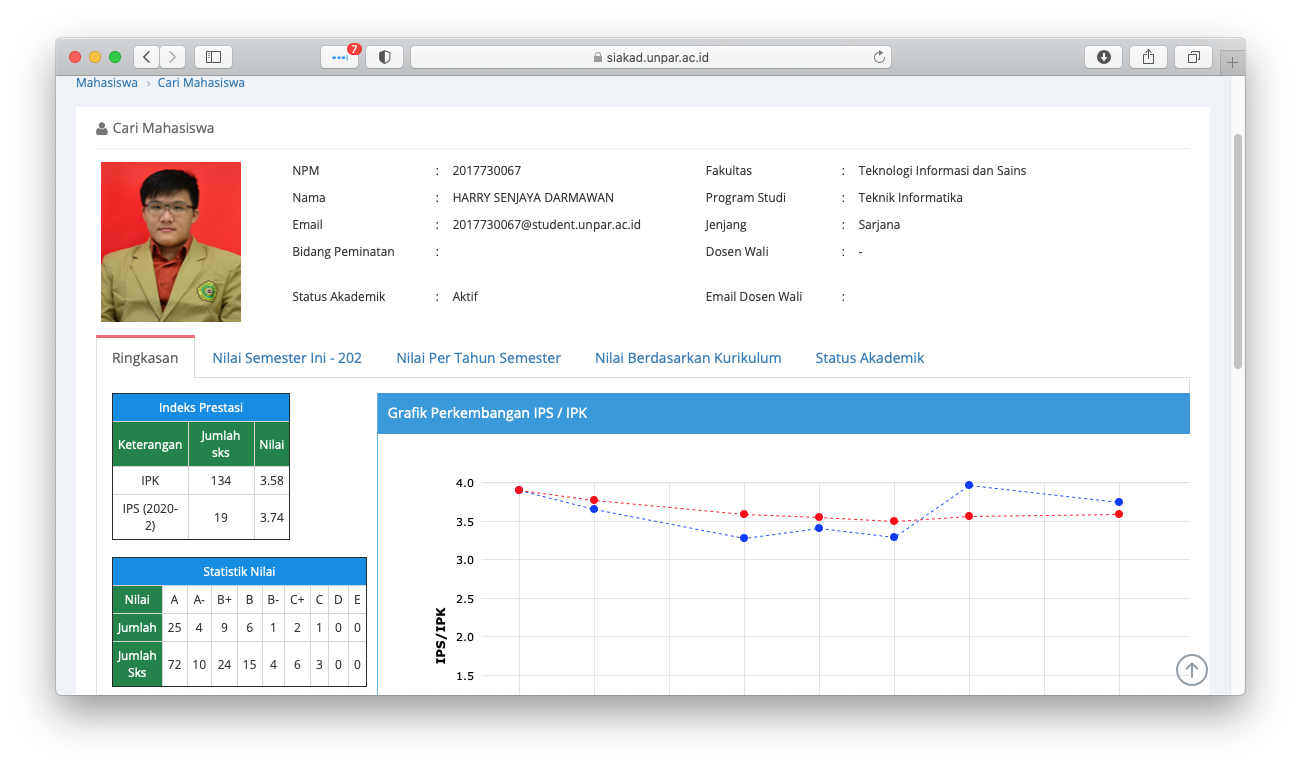
\includegraphics[scale=0.35]{Gambar/siakad_akademik_ringkasan.png}
    \caption{Tangkapan Layar Tab Ringkasan Akademik}
    \label{fig:3_siakad_akademik_ringkasan}
\end{figure}

\paragraph{Nilai Semester Ini} Tab ini berisi data nilai dari kuliah-kuliah yang sedang diambil pada semester ini (Gambar \ref{fig:3_siakad_akademik_nilaisemesterini}).

\begin{figure}[H]
    \centering
    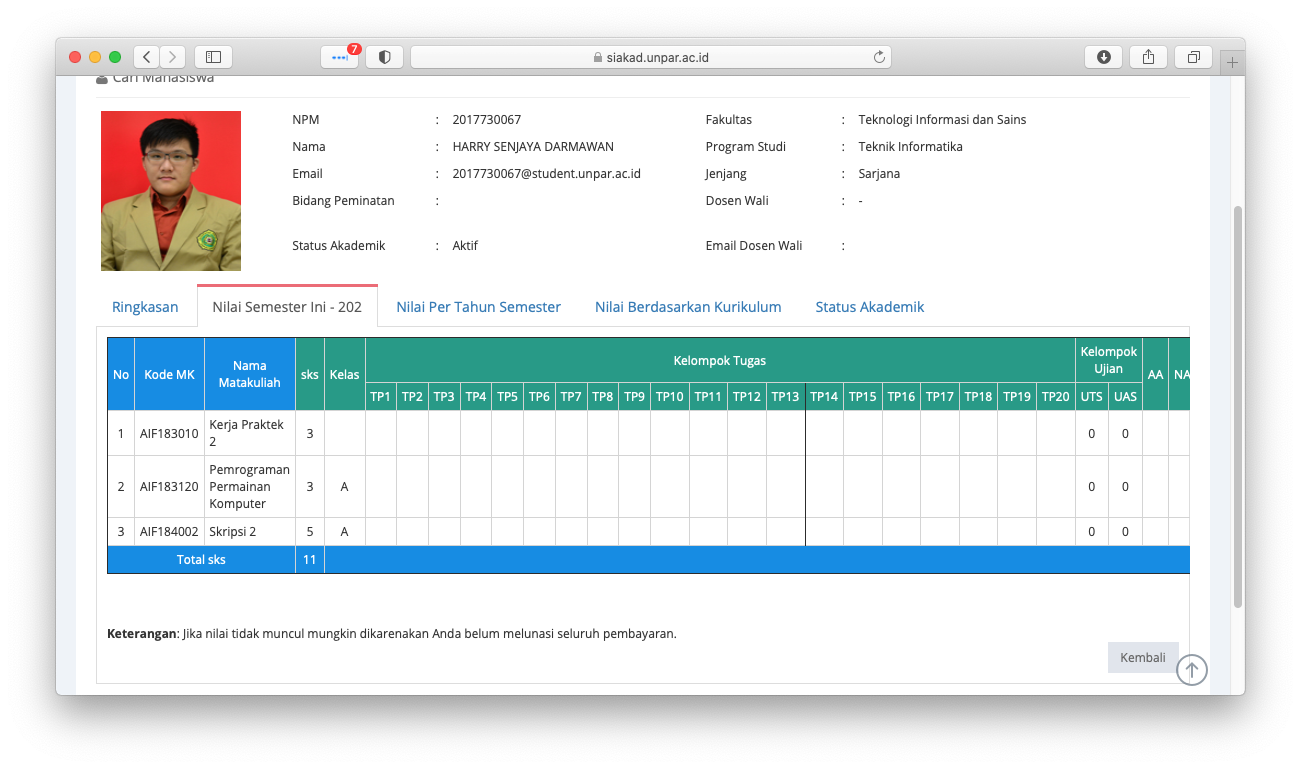
\includegraphics[scale=0.35]{Gambar/siakad_akademik_nilaisemesterini.png}
    \caption{Tangkapan Layar Tab Nilai Semester Ini}
    \label{fig:3_siakad_akademik_nilaisemesterini}
\end{figure}

\paragraph{Nilai Per Tahun Semester} Tab ini berisi data nilai mahasiswa, dibagi per tahun semester (Gambar \ref{fig:3_siakad_akademik_nilaipertahunsemester}).

\begin{figure}[H]
    \centering
    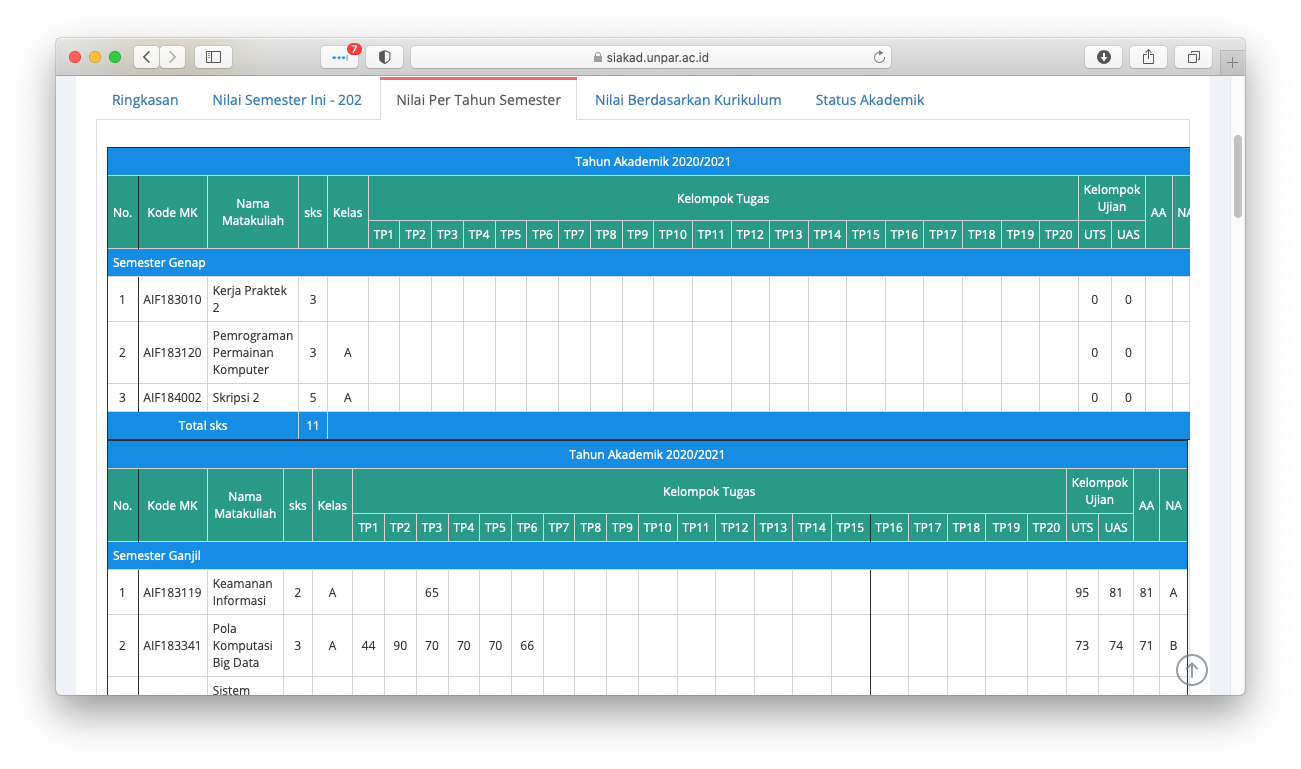
\includegraphics[scale=0.35]{Gambar/siakad_akademik_nilaipertahunsemester.png}
    \caption{Tangkapan Layar Tab Nilai Per Tahun Semester}
    \label{fig:3_siakad_akademik_nilaipertahunsemester}
\end{figure}

\paragraph{Nilai Berdasarkan Kurikulum} Tab ini berisi data nilai mahasiswa, dibagi berdasarkan acuan linimasa kurikulum (Gambar \ref{fig:3_siakad_akademik_nilaiberdasarkankurikulum}).

\begin{figure}[H]
    \centering
    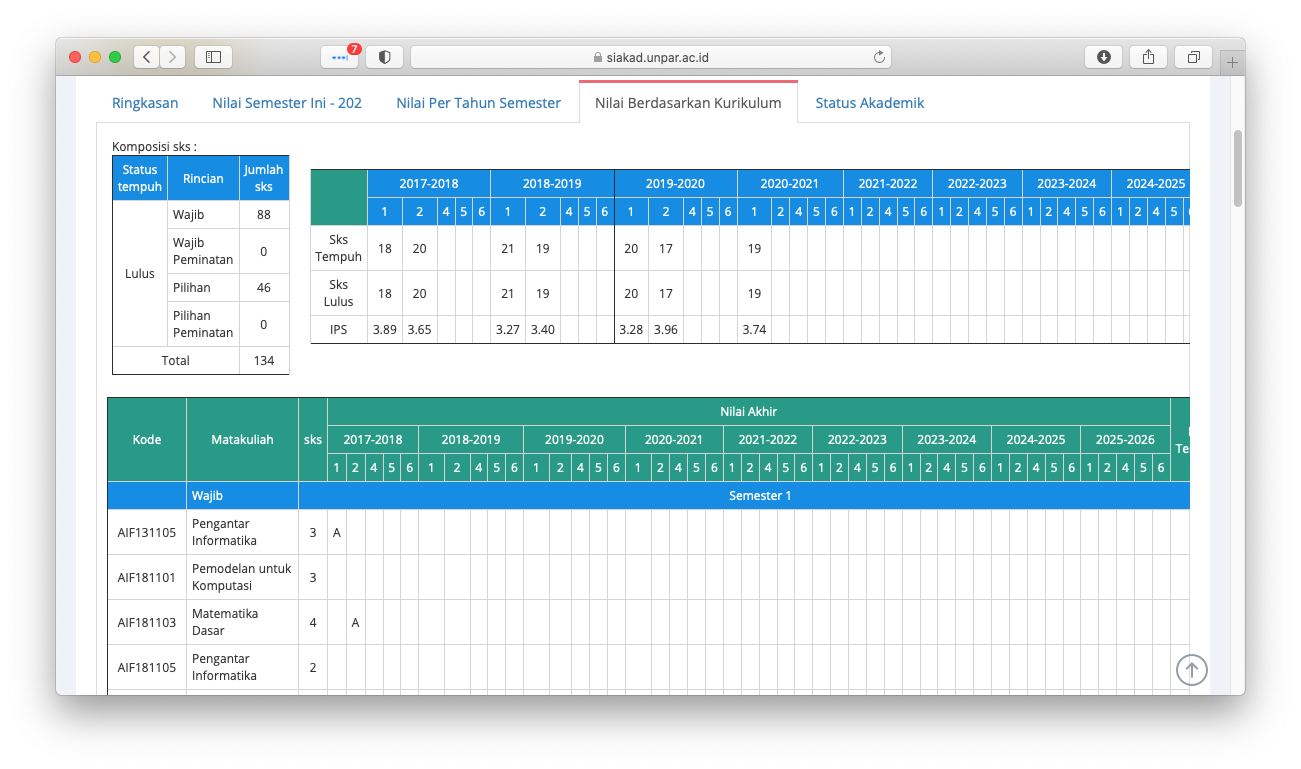
\includegraphics[scale=0.35]{Gambar/siakad_akademik_nilaiberdasarkankurikulum.png}
    \caption{Tangkapan Layar Tab Nilai Berdasarkan Kurikulum}
    \label{fig:3_siakad_akademik_nilaiberdasarkankurikulum}
\end{figure}

\paragraph{Status Akademik} Tab ini berisi riwayat status akademik mahasiswa, termasuk perubahan dosen wali (Gambar \ref{fig:3_siakad_akademik_statusakademik}).

\begin{figure}[H]
    \centering
    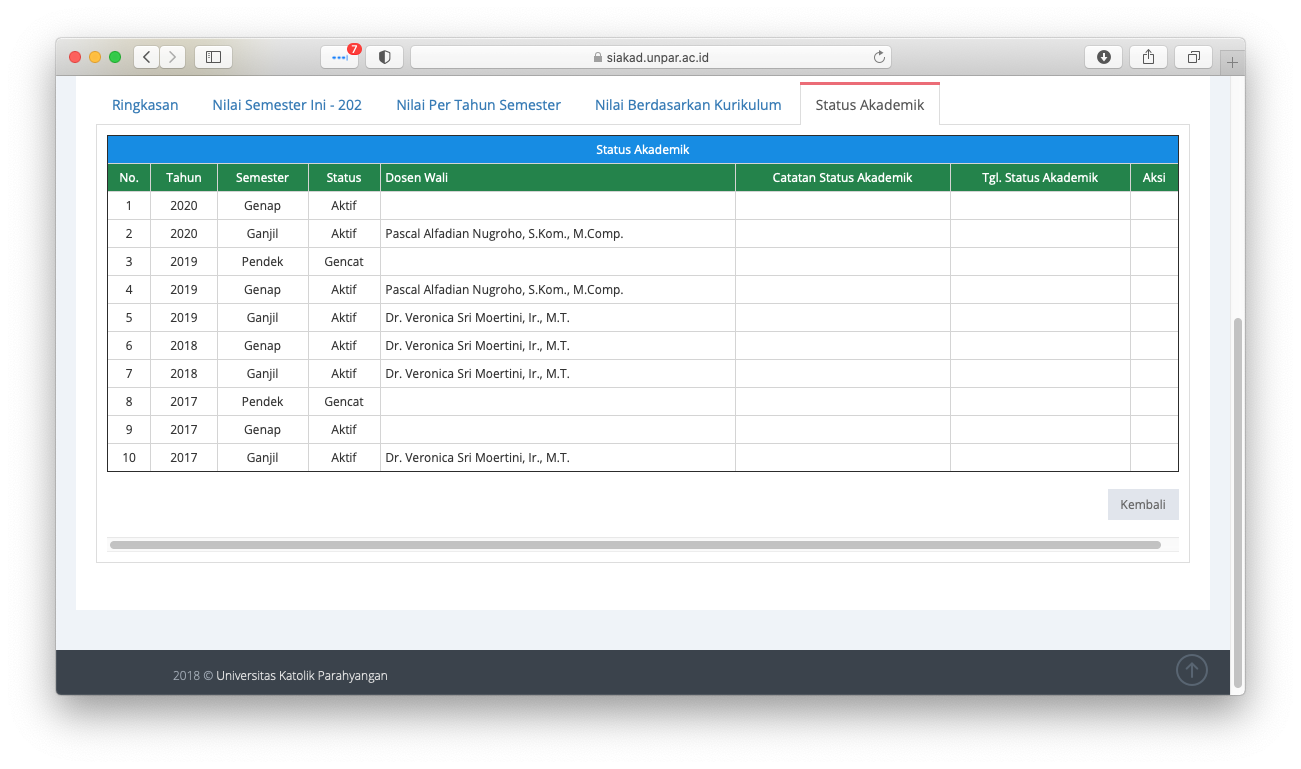
\includegraphics[scale=0.35]{Gambar/siakad_akademik_statusakademik.png}
    \caption{Tangkapan Layar Tab Status Akademik}
    \label{fig:3_siakad_akademik_statusakademik}
\end{figure}

\subsection{Pra Kuliah}

Bagian ini tidak dijelaskan karena tidak berkaitan dengan informasi mahasiswa.

\subsection{Perkuliahan}

Bagian ini tidak dijelaskan karena tidak berkaitan dengan informasi mahasiswa.

\subsection{Ujian}

Bagian ini tidak dijelaskan karena tidak berkaitan dengan informasi mahasiswa.

\subsection{Nilai}

Bagian ini tidak dijelaskan karena tidak berkaitan dengan informasi mahasiswa.

\subsection{Evaluasi}

Pada menu Evaluasi, hanya ada satu submenu untuk dosen, yaitu Laporan Evaluasi, yang memiliki satu subsubmenu juga, yaitu Daftar Perkembangan Studi. Di halaman ini, dosen dapat mencari data mahasiswa walinya, berupa Daftar Perkembangan Studi dalam bentuk PDF, seperti ditunjukkan pada Gambar \ref{fig:3_siakad_dps_detail}.

\begin{figure}[H]
    \centering
    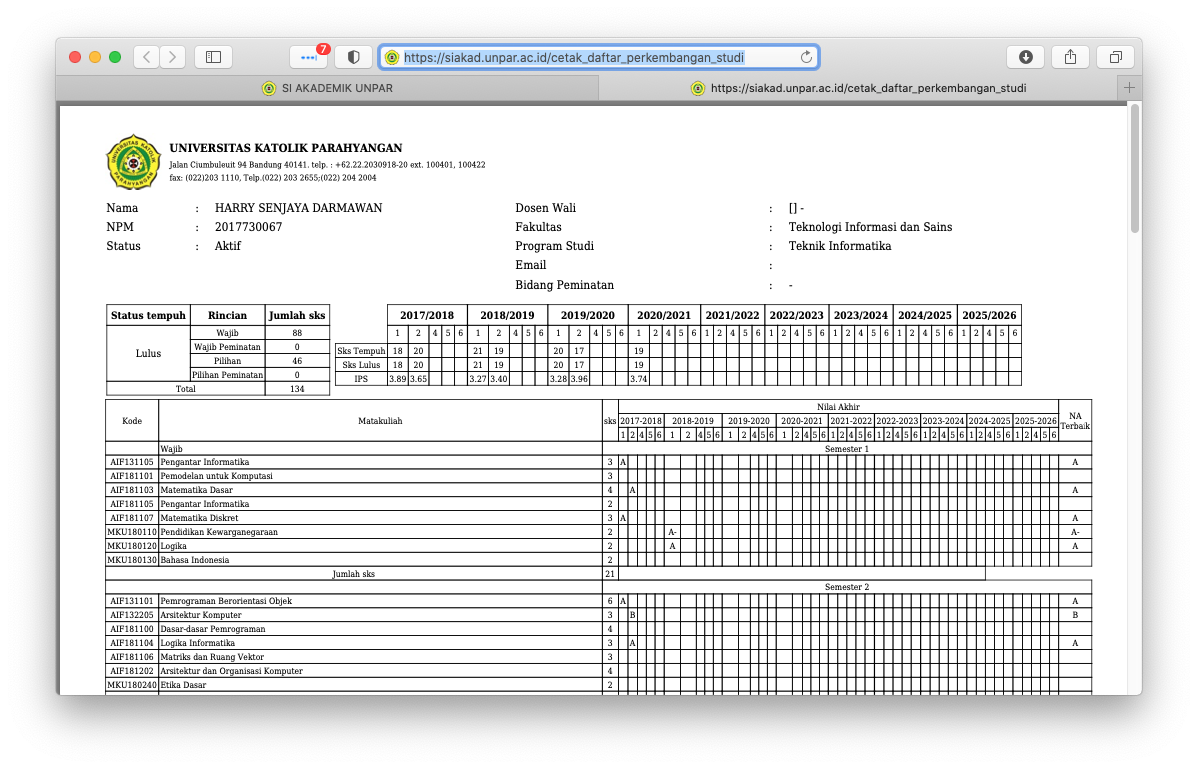
\includegraphics[scale=0.35]{Gambar/siakad_dps_detail.png}
    \caption{Tangkapan Layar PDF Daftar Perkembangan Studi}
    \label{fig:3_siakad_dps_detail}
\end{figure}
\subsection{Skripsi}

Bagian ini tidak dijelaskan karena tidak berkaitan dengan informasi mahasiswa.

\subsection{Sidang}

Bagian ini tidak dijelaskan karena tidak berkaitan dengan informasi mahasiswa.

\subsection{Kelulusan}

Bagian ini tidak dijelaskan karena tidak berkaitan dengan informasi mahasiswa.

\subsection{Pengumuman}

Bagian ini tidak dijelaskan karena tidak berkaitan dengan informasi mahasiswa.

\section{Data yang Dibutuhkan untuk \textit{Screensaver}}

\subsection{Portal Akademik Mahasiswa}

\subsubsection{Halaman Utama}
Pada Halaman Utama Portal Akademik Mahasiswa terdapat nama lengkap dan foto dari mahasiswa tersebut yang dapat diambil dan digunakan (Gambar \ref{fig:3_home} dengan kotak merah). Nama mahasiswa dapat diambil dengan mencari elemen \texttt{"div"} yang memiliki kelas \texttt{"namaUser d-none d-lg-block mr-3"}, sehingga kueri css yang dihasilkan adalah \texttt{"div[class=namaUser d-none d-lg-block mr-3]"}. Foto mahasiswa dapat diambil dengan mencari elemen \texttt{"img"} yang memiliki kelas \texttt{"img-fluid fotoProfil"}, sehingga kueri css yang dihasilkan adalah \texttt{"img[class=img-fluid fotoProfil]"}.
Terdapat beberapa perubahan (Kode \ref{diff_halaman_utama}) yang perlu dilakukan terhadap skripsi Andrianto Sugiarto \cite{ifstupor}: 

\begin{enumerate}
    \item Menghapus pemanggilan fungsi validateTLSCertificates() dikarenakan sudah \textit{deprecated} \cite{jsoup}.
    \item Sebelumnya semester yang sedang dijalani mahasiswa diambil dari menu FRS/PRS, namun karena terdapat perubahan dimana menu FRS/PRS tidak menuju ke Portal Akademik Mahasiswa melainkan menuju ke \url{https://restu.unpar.ac.id/frs_prs}, sehingga perlu melakukan \textit{login} kembali apabila mengakses \textit{URL} tersebut, maka semester yang sedang dijalani mahasiswa diambil dari menu Nilai. Dengan begitu, kueri css untuk pengambilan semester yang sedang dijalani juga perlu diubah, yaitu dengan mencari elemen \texttt{"select"} yang memiliki kelas \texttt{"custom-select mr-3"}, sehingga kueri css yang dihasilkan adalah \texttt{"select[class=custom-select mr-3]"}. Kemudian mengolah data yang didapat sehingga dapat dijadikan objek bertipe \texttt{TahunSemester} sesuai dengan SIAModels.
\end{enumerate}

\begin{lstlisting}[language=diff, caption=Perubahan Implementasi Jsoup Halaman Utama, label=diff_halaman_utama]
@@ -96,24 +96,22 @@ public class Scraper {
         Connection connection = Jsoup.connect(HOME_URL);
         connection.cookie("ci_session", phpsessid);
         connection.timeout(0);
-        connection.validateTLSCertificates(false);
         connection.method(Connection.Method.GET);
         Response resp = connection.execute();
         Document doc = resp.parse();
         String nama = doc.select("div[class=namaUser d-none d-lg-block mr-3]").text();
         mhs.setNama(nama.substring(0, nama.indexOf(mhs.getEmailAddress())));
         Element photo = doc.select("img[class=img-fluid fotoProfil]").first();
         String photoPath = photo.attr("src");
         mhs.setPhotoPath(photoPath);
-        connection = Jsoup.connect(FRSPRS_URL);
+        connection = Jsoup.connect(NILAI_URL);
         connection.cookie("ci_session", phpsessid);
         connection.timeout(0);
-        connection.validateTLSCertificates(false);
         connection.method(Connection.Method.GET);
         resp = connection.execute();
         doc = resp.parse();
-        String curr_sem = doc.select(".custom-selectContent span").text();
-        String[] sem_set = parseSemester(curr_sem);
+        Elements curr_sem = doc.select("select[class=custom-select mr-3]");
+        String[] sem_set = parseSemester(curr_sem.first().child(curr_sem.first().childrenSize() - 1).text());
         TahunSemester currTahunSemester = new TahunSemester(Integer.parseInt(sem_set[0]),
                 Semester.fromString(sem_set[1]));
         return currTahunSemester;
@@ -214,7 +212,7 @@ public class Scraper {
     }

     public String[] parseSemester(String sem_raw) {
-        String[] sem_set = sem_raw.split("/")[0].split("-");
+        String[] sem_set = sem_raw.split("/")[0].split(" ");
         return new String[]{sem_set[1].trim(), sem_set[0].trim()};
     }
\end{lstlisting}

\subsubsection{Halaman Profil}
Pada Halaman Profil (Gambar \ref{fig:3_profil} dengan kotak merah), tanggal lahir mahasiswa akan diambil untuk ditampilkan pada \textit{screensaver}. Implementasi jsoup tersebut belum diimplementasikan pada skripsi Andrianto Sugiarto \cite{ifstupor}, sehingga perlu dilakukan penambahan fitur untuk mengambil data tersebut. Tanggal lahir mahasiswa dapat diambil dengan mencari elemen \texttt{"div"} yang memiliki kelas \texttt{"offset-md-1 col-md-10 col-12 headerWrapper my-0 border-bottom"}, sehingga kueri css yang dihasilkan adalah \texttt{"div[class=offset-md-1 col-md-10 col-12 headerWrapper my-0 border-bottom]"}.


\subsubsection{Halaman Daftar Perkembangan Studi}
Pada Halaman Daftar Perkembangan Studi (Gambar \ref{fig:3_dps_1} dan \ref{fig:3_dps_2} dengan kotak merah), data yang dapat dimanfaatkan dari halaman ini adalah IPK, IPS, jumlah sks yang lulus, dan jumlah sks yang ditempuh. Namun, pada SIAModels sudah terdapat \textit{method} yang melakukan kalkulasi untuk mendapatkan data-data tersebut, sehingga tidak perlu dilakukan pengambilan data menggunakan jsoup. Untuk dapat memanfaatkan \textit{method} tersebut diperlukan seluruh riwayat mata kuliah dan nilai yang pernah ditempuh mahasiswa, sehingga perlu dilakukan pengambilan data menggunakan jsoup.  Implementasi pengambilan data tersebut sudah diimplementasikan sebelumnya pada skripsi Andrianto Sugiarto \cite{ifstupor}. Proses dari pengambilan data tersebut yaitu:
    \begin{itemize}
        \item Mengambil data nilai berdasarkan tahun dan semester dengan mencari elemen \texttt{"select"} yang memiliki id \texttt{"dropdownSemester"}, dan memiliki kelas \texttt{"custom-select mr-3"} sehingga kueri css yang dihasilkan adalah \texttt{"select\#dropdownSemester.custom-select.mr-3"}.
        \label{multipleRequest}
        \item Dikarenakan perlunya melakukan koneksi berkali-kali sebanyak semester yang telah ditempuh mahasiswa, sehingga dibutuhkan waktu yang tidak sebentar. Karena pada halaman nilai tidak dapat menampilkan seluruh semester seperti Portal Akademik Mahasiswa yang lama, sehingga untuk mengatasi masalah ini dibuat menjadi paralel. Untuk itu dibuat kelas yang mengimplementasikan kelas \textit{interface} \texttt{Runnable}, yaitu kelas \texttt{MultipleRequest}. Kelas inilah yang melakukan koneksi ke setiap semester yang telah ditempuh mahasiswa, dan mengambil data-data tersebut.
    \end{itemize}
    Namun, terdapat beberapa perubahan (Kode \ref{diff_halaman_dps}) yang perlu dilakukan:
    \begin{enumerate}
        \item Menghapus pemanggilan fungsi validateTLSCertificates() dikarenakan sudah \textit{deprecated} \cite{jsoup}.
        \item Indeks yang digunakan untuk melakukan kueri css berubah, sehingga untuk mengantisipasi tersebut, indeks yang digunakan menjadi \textit{size} dari kueri css dikurangi 1.
    \end{enumerate}
        
        
        \begin{lstlisting}[language=diff, caption=Perubahan Implementasi Jsoup Halaman Daftar Perkembangan Studi, label=diff_halaman_dps]
@@ -50,7 +50,7 @@ public class MultipleRequest implements Runnable {
             Connection.Response resp = connection.execute();
             Document doc = resp.parse();

-            Element script = doc.select("script").get(10);
+            Element script = doc.select("script").get(doc.select("script").size()-1);
             String scriptDataMataKuliah = script.html().substring(script.html().indexOf("var data_mata_kuliah = [];"), script.html().indexOf("var data_angket = [];"));
             engine.eval(scriptDataMataKuliah);
             ScriptObjectMirror dataMataKuliah = (ScriptObjectMirror) engine.get("data_mata_kuliah");
             
@@ -131,7 +131,6 @@ public class Scraper {
         Connection connection = Jsoup.connect(NILAI_URL);
         connection.cookie("ci_session", phpsessid);
         connection.timeout(0);
-        connection.validateTLSCertificates(false);
         connection.method(Connection.Method.POST);
         Response resp = connection.execute();
         Document doc = resp.parse();
        \end{lstlisting}
        
        
\subsubsection{Halaman TOEFL}
Pada Halaman TOEFL (Gambar \ref{fig:3_toefl} dengan kotak merah), riwayat skor TOEFL dapat diambil dengan mencari elemen \texttt{"table"} yang memiliki elemen \texttt{"tbody"} didalamnya, serta memiliki elemen \texttt{"tr"} didalam elemen \texttt{"tbody"}.
Terdapat beberapa perubahan yang terjadi pada halaman TOEFL semenjak skripsi Andrianto Sugiarto \cite{ifstupor}, yang mengakibatkan perlunya perubahan (Kode \ref{diff_toefl}) terhadap implementasi jsoup:

    \begin{enumerate}
        \item Menghapus pemanggilan fungsi validateTLSCertificates() dikarenakan sudah \textit{deprecated} \cite{jsoup}.
        \item Perubahan format tanggal TOEFL pada Portal Akademik Mahasiswa menjadi dd-mm-yyyy.
    \end{enumerate}
       
        \begin{lstlisting}[language=diff, caption=Perubahan Implementasi Jsoup TOEFL, label=diff_toefl]
@@ -174,7 +174,6 @@ public class Scraper {
         Connection connection = Jsoup.connect(TOEFL_URL);
         connection.cookie("ci_session", phpsessid);
         connection.timeout(0);
-        connection.validateTLSCertificates(false);
         connection.method(Connection.Method.POST);
         Response resp = connection.execute();
         Document doc = resp.parse();
@@ -183,45 +182,7 @@ public class Scraper {
             for (int i = 0; i < nilaiTOEFL.size(); i++) {
                 Element nilai = nilaiTOEFL.get(i).select("td").get(5);
                 Element tgl_toefl = nilaiTOEFL.get(i).select("td").get(1);
-                String[] tanggal = tgl_toefl.text().split(" ");
-                switch (tanggal[1].toLowerCase()) {
-                    case "januari":
-                        tanggal[1] = "1";
-                        break;
-                    case "februari":
-                        tanggal[1] = "2";
-                        break;
-                    case "maret":
-                        tanggal[1] = "3";
-                        break;
-                    case "april":
-                        tanggal[1] = "4";
-                        break;
-                    case "mei":
-                        tanggal[1] = "5";
-                        break;
-                    case "juni":
-                        tanggal[1] = "6";
-                        break;
-                    case "juli":
-                        tanggal[1] = "7";
-                        break;
-                    case "agustus":
-                        tanggal[1] = "8";
-                        break;
-                    case "september":
-                        tanggal[1] = "9";
-                        break;
-                    case "oktober":
-                        tanggal[1] = "10";
-                        break;
-                    case "november":
-                        tanggal[1] = "11";
-                        break;
-                    case "desember":
-                        tanggal[1] = "12";
-                        break;
-                }
+                String[] tanggal = tgl_toefl.text().split("-");

                 LocalDate localDate = LocalDate.of(Integer.parseInt(tanggal[2]), Integer.parseInt(tanggal[1]),
                         Integer.parseInt(tanggal[0]));
        \end{lstlisting}

\subsection{SIAKAD}

\textit{Subbab ini ditulis oleh dosen pembimbing.}

\subsubsection{Mendapatkan daftar mahasiswa}

Untuk mendapatkan daftar mahasiswa, bisa memanfaatkan halaman ``Cari Mahasiswa''. Caranya dengan mensimulasikan penekanan tombol ``Cari'' dengan parameter \textit{default}, yang akan menampilkan daftar mahasiswa dari dosen wali yang bersangkutan. Hasilnya dalam bentuk tabel dan di-\textit{parsing}, dengan ketentuan sebagai berikut:

\begin{enumerate}
    \item NPM tersedia pada kolom kedua.
    \item Nama Mahasiswa tersedia pada kolom ketiga.
    \item Kolom-kolom lainnya diabaikan.
\end{enumerate}

\subsubsection{Mendapatkan detail mahasiswa}

\paragraph{Riwayat Nilai} Pada SIAKAD, riwayat nilai mahasiswa tersedia pada beberapa halaman:

\begin{enumerate}
    \item \textbf{Nilai Per Tahun Semester} berisikan tabel nilai yang dibagi per tahun semester. Data dari halaman inilah yang dipakai untuk mendapatkan nilai mahasiswa, mencakup: kode dan nama mata kuliah, SKS, kelas, TP1 s.d. TP20, UTS, UAS, AA, dan NA.
    \item \textbf{Nilai Berdasarkan Kurikulum} berisikan tabel nilai yang dibagi berdasarkan linimasa kurikulum. Data ini kurang cocok dipakai karena tidak mengandung nilai tugas dan ujian, hanya nilai akhir saja.
    \item \textbf{Evaluasi} berisikan tabel nilai lengkap dalam bentuk Daftar Perkembangan Studi dengan format PDF. Data ini sulit diekstraksi karena tidak dalam bentuk HTML.
\end{enumerate}

Kesimpulannya, riwayat nilai diambil dari halaman ``Nilai Per Tahun Semester''.

\paragraph{Data Diri} Pada SIAKAD, data diri dapat diambil dari halaman ``Data Diri'', tab identitas mahasiswa. Foto tersedia dalam bentuk Data URL\footnote{\url{https://developer.mozilla.org/en-US/docs/Web/HTTP/Basics_of_HTTP/Data_URIs}} yang di-\textit{encode} dalam format \textit{base64}. Data-data diri lainnya dapat diambil dengan cukup sederhana dari berbagai elemen yang ada di tab tersebut.


\section{Analisis Sistem \textit{Screensaver}}

\subsection{Diagram \textit{Use Case Screensaver}}

\begin{figure}[H]
	\centering
	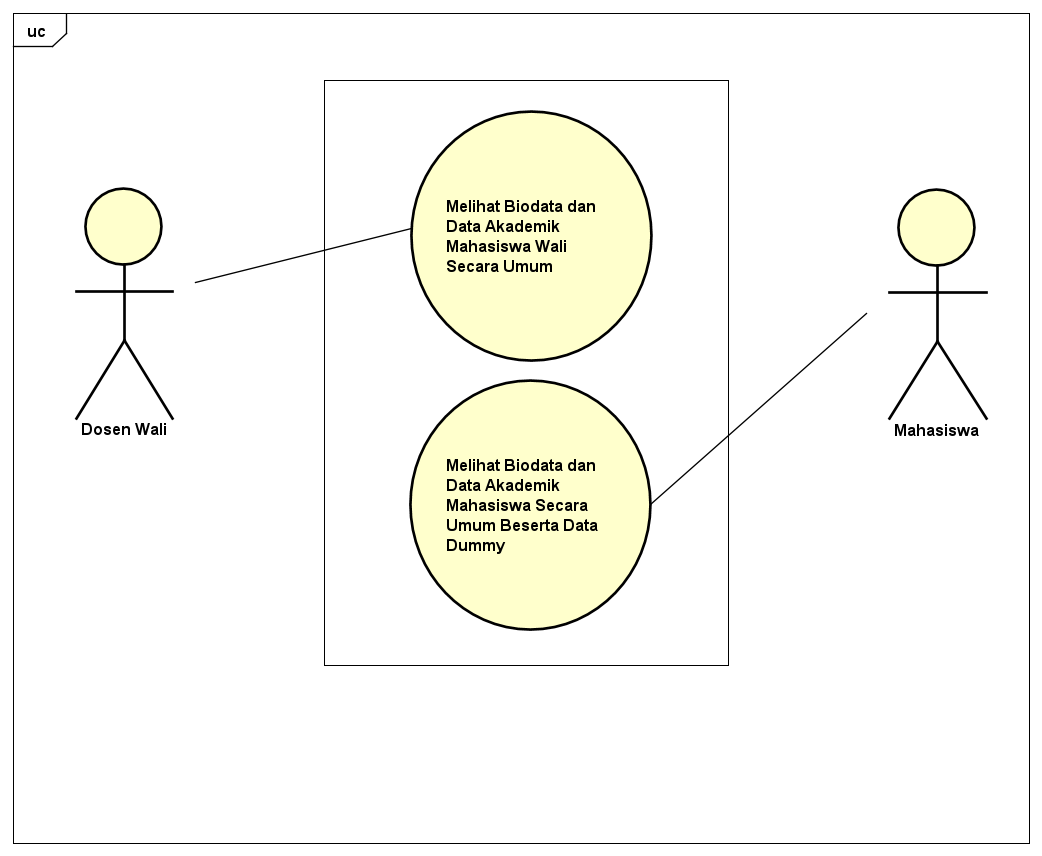
\includegraphics[scale=0.45]{Gambar/UseCase.png}
	\caption{Diagram \textit{Use Case Screensaver}}
	\label{fig:3_usecase_diagram}
\end{figure}
    
Pada diagram \textit{use case screensaver} (Gambar \ref{fig:3_usecase_diagram}) terdapat 1 fitur utama
dari \textit{screensaver} yaitu, melihat biodata dan data akademik mahasiswa secara umum. Dimana biodata yang dimaksud adalah nama, angkatan, tanggal lahir. Serta data akademik yang dimaksud adalah status, email, nilai TOEFL, IPS, IPK, SKS lulus, SKS tempuh mahasiswa.
